\chapter[Introduction to the FDTD Method]{Introduction to
the Finite-Difference Time-Domain Method: FDTD in 1D
\label{chap:fdtdIntro}} 

%\setcounter{page}{1}

\renewcommand{\thefootnote}{\fnsymbol{footnote}}
\footnotetext{Lecture notes by John Schneider.  {\tt
fdtd-intro.tex}}

\section{Introduction}

The finite-difference time-domain (FDTD) method is arguably the
simplest, both conceptually and in terms of implementation, of the
full-wave techniques used to solve problems in electromagnetics.  It
can accurately tackle a wide range of problems.  However, as with all
numerical methods, it does have its share of artifacts and the
accuracy is contingent upon the implementation.  The FDTD method can
solve complicated problems, but it is generally computationally
expensive.  Solutions may require a large amount of memory and
computation time.  The FDTD method loosely fits into the category of
``resonance region'' techniques, i.e., ones in which the
characteristic dimensions of the domain of interest are somewhere on
the order of a wavelength in size.  If an object is very small
compared to a wavelength, quasi-static approximations generally
provide more efficient solutions.  Alternatively, if the wavelength is
exceedingly small compared to the physical features of interest,
ray-based methods or other techniques may provide a much more
efficient way to solve the problem.

The FDTD method employs finite differences as approximations to both
the spatial and temporal derivatives that appear in Maxwell's
equations (specifically Ampere's and Faraday's laws).  Consider the
Taylor series expansions of the function $f(x)$ expanded about the
point $x_0$ with an offset of $\pm\delta/2$:
\begin{eqnarray}
  f\!\left(x_0+\frac{\delta}{2}\right) &=&
    f(x_0) + \frac{\delta}{2} f'(x_0) +
        \frac{1}{2!}\left(\frac{\delta}{2}\right)^2 f''(x_0) + 
        \frac{1}{3!}\left(\frac{\delta}{2}\right)^3 f'''(x_0) + \ldots,
  \\
  f\!\left(x_0-\frac{\delta}{2}\right) &=&
    f(x_0) - \frac{\delta}{2} f'(x_0) +
        \frac{1}{2!}\left(\frac{\delta}{2}\right)^2 f''(x_0) -
        \frac{1}{3!}\left(\frac{\delta}{2}\right)^3 f'''(x_0) + \ldots
\end{eqnarray}
where the primes indicate differentiation.  Subtracting the second
equation from the first yields
\begin{equation}
  f\!\left(x_0+\frac{\delta}{2}\right) -
  f\!\left(x_0-\frac{\delta}{2}\right) = 
   \delta f'(x_0) +
        \frac{2}{3!}\left(\frac{\delta}{2}\right)^3 f'''(x_0) + \ldots
\end{equation}
Dividing by $\delta$ produces
\begin{equation}
  \frac{f\!\left(x_0+\frac{\delta}{2}\right) -
        f\!\left(x_0-\frac{\delta}{2}\right)}{\delta} = 
   f'(x_0) +
        \frac{1}{3!}\frac{\delta^2}{2^2} f'''(x_0) + \ldots
\end{equation}
Thus the term on the left is equal to the derivative of the function
at the point $x_0$ plus a term which depends on $\delta^2$ plus an
infinite number of other terms which are not shown.  For the terms
which are not shown, the next would depend on $\delta^4$ and all
subsequent terms would depend on even higher powers of $\delta$.
Rearranging slightly, this relationship is often stated as
\begin{equation}
  \left.\frac{df(x)}{dx}\right|_{x=x_0} = 
  \frac{f\!\left(x_0+\frac{\delta}{2}\right) -
        f\!\left(x_0-\frac{\delta}{2}\right)}{\delta} + O(\delta^2).
\end{equation}
The ``big-Oh'' term represents all the terms that are not explicitly
shown and the value in parentheses, i.e., $\delta^2$, indicates the
lowest order of $\delta$ in these hidden terms.  If $\delta$ is
sufficiently small, a reasonable approximation to the derivative may
be obtained by simply neglecting all the terms represented by the
``big-Oh'' term.  Thus, the central-difference approximation is given
by
\begin{equation}
  \left.\frac{df(x)}{dx}\right|_{x=x_0} \approx
  \frac{f\!\left(x_0+\frac{\delta}{2}\right) -
        f\!\left(x_0-\frac{\delta}{2}\right)}{\delta}.
\end{equation}
Note that the central difference provides an approximation of the
derivative of the function at $x_0$, but the function is not actually
sampled there.  Instead, the function is sampled at the neighboring
points $x_0+\delta/2$ and $x_0-\delta/2$.  Since the lowest power of
$\delta$ being ignored is second order, the central difference is said
to have second-order accuracy or second-order behavior.  This implies
that if $\delta$ is reduced by a factor of $10$, the error in the
approximation should be reduced by a factor of $100$ (at least
approximately).  In the limit as $\delta$ goes to zero, the
approximation becomes exact.

One can construct higher-order central differences.  In order to get
higher-order behavior, more terms, i.e., more sample points, must be
used.  Appendix \ref{ap:diff} presents the construction of a
fourth-order central difference.  The use of higher-order central
differences in FDTD schemes is certainly possible, but there are some
complications which arise because of the increased ``stencil'' of the
difference operator.  For example, when a PEC is present, it is
possible that the difference operator will extend into the PEC
prematurely or it may extend to the other side of a PEC sheet.
Because of these types of issues, we will only consider the use of
second-order central difference.

\section{The Yee Algorithm}

The FDTD algorithm as first proposed by Kane Yee in 1966 employs
second-order central differences.  The algorithm can be summarized as
follows:
\begin{enumerate}
\item Replace all the derivatives in Ampere's and Faraday's laws with
finite differences.  Discretize space and time so that the electric and
magnetic fields are staggered in both space and time.

\item Solve the resulting difference equations to obtain ``update
equations'' that express the (unknown) future fields in terms of
(known) past fields.

\item Evaluate the magnetic fields one time-step into the future so
they are now known (effectively they become past fields).

\item Evaluate the electric fields one time-step into the future so
they are now known (effectively they become past fields). 

\item Repeat the previous two steps until the fields have been
obtained over the desired duration.
\end{enumerate}
At this stage, the summary is probably a bit too abstract.  One really
needs an example to demonstrate the simplicity of the method.
However, developing the full set of three-dimensional equations would
be overkill and thus the algorithm will first be presented in
one-dimension.  As you will see, the extension to higher dimensions is
quite simple.

\section{Update Equations in 1D \label{sec:update}}

Consider a one-dimensional space where there are only variations in
the $x$ direction.  Assume that the electric field only has a $z$
component.  In this case Faraday's law can be written
\begin{equation}
  -\mu \frac{\partial \Hvec}{\partial t} =
  \nabla \times \Evec =
  \left|
  \begin{array}{ccc}
     \unitvec{x} & \unitvec{y} & \unitvec{z} \\
     \frac{\partial}{\partial x} & 0 & 0 \\
     0 & 0 & E_z
  \end{array}
  \right|
  = -\unitvec{y}\frac{\partial E_z}{\partial x}.
 \label{eq:faradayVec}
\end{equation}
Thus $H_y$ must be the only non-zero component of the magnetic field
which is time varying.  (Since the right-hand side of this equation
has only a $y$ component, the magnetic field may have non-zero
components in the $x$ and $z$ directions, but they must be static.  We
will not be concerned with static fields here.)  Knowing this,
Ampere's law can be written
\begin{equation}
  \epsilon \frac{\partial \Evec}{\partial t} =
  \nabla \times \Hvec =
  \left|
  \begin{array}{ccc}
     \unitvec{x} & \unitvec{y} & \unitvec{z} \\
     \frac{\partial}{\partial x} & 0 & 0 \\
     0 & H_y & 0
  \end{array}
  \right|
  = \unitvec{z}\frac{\partial H_y}{\partial x}.
 \label{eq:ampereVec}
\end{equation}
The two scalar equations obtained from \refeq{eq:faradayVec} and
\refeq{eq:ampereVec} are
\begin{eqnarray}
  \mu \frac{\partial H_y}{\partial t} &=&
    \frac{\partial E_z}{\partial x},  \label{eq:faradayScalar}
  \\
  \epsilon \frac{\partial E_z}{\partial t} &=&
    \frac{\partial H_y}{\partial x}. \label{eq:ampereScalar}
\end{eqnarray}
The first equation gives the temporal derivative of the magnetic field
in terms of the spatial derivative of the electric field.  Conversely,
the second equation gives the temporal derivative of the electric
field in terms of the spatial derivative of the magnetic field.  As
will be shown, the first equation will be used to advance the magnetic
field in time while the second will be used to advance the electric
field.  A method in which one field is advanced and then the other,
and then the process is repeated, is known as a leap-frog method.

The next step is to replace the derivatives in
\refeq{eq:faradayScalar} and \refeq{eq:ampereScalar} with finite
differences.  To do this, space and time need to be discretized.  The
following notation will be used to indicate the location where the
fields are sampled in space and time
\begin{eqnarray}
  E_z(x,t) \!&=&\! E_z(m\Delx, q\Delt) = \fdtd{E_z}{m}{q}, \\
  H_y(x,t) \!&=&\! H_y(m\Delx, q\Delt) = \fdtd{H_y}{m}{q},
\end{eqnarray}
where $\Delx$ is the spatial offset between sample points and $\Delt$
is the temporal offset.  The index $m$ corresponds to the spatial
step, effectively the spatial location, while the index $q$
corresponds to the temporal step.  When written as a superscript $q$
still represents the temporal step---it is not an exponent.  When
implementing FDTD algorithms we will see that the spatial indices are
used as array indices while the temporal index, which is essentially a
global parameter, is not explicitly specified for each field location.
Hence, it is reasonable to keep the spatial indices as an explicit
argument while indicating the temporal index separately.

Although we only have one spatial dimension, time can be thought of as
another dimension.  Thus this is effectively a form of two-dimensional
problem.  The question now is: How should the electric and magnetic
field sample points, also known as nodes, be arranged in space and
time?  The answer is shown in Fig.\ \ref{fig:spaceTime}.
\begin{figure}
  \begin{center}
  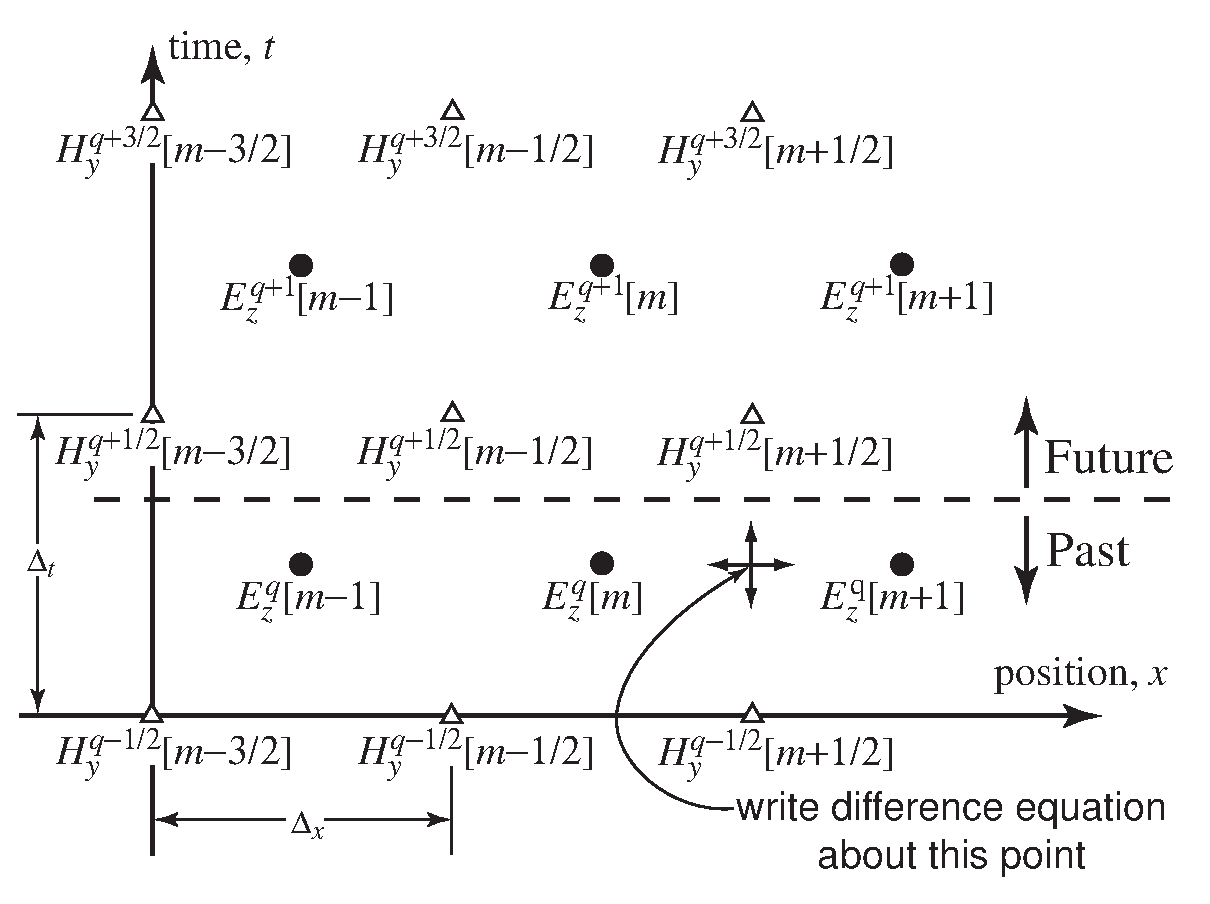
\epsfig{width=4.6in,file=Figures/Fdtd-intro/space-time-fdtd-update-new.eps}
  \end{center}
  \caption{The arrangement of electric- and magnetic-field nodes in
  space and time.  The electric-field nodes are shown as circles and
  the magnetic-field nodes as triangles.  The indicated point is where the
  difference equation is expanded to obtain an update equation for
  $H_y$.}
  \label{fig:spaceTime}
\end{figure}
The electric-field nodes are shown as circles and the magnetic-field
nodes as triangles.  Assume that all the fields below the dashed line
are known---they are considered to be in the past---while the fields
above the dashed line are future fields and hence unknown.  The FDTD
algorithm provides a way to obtain the future fields from the past
fields.

As indicated in Fig.\ \ref{fig:spaceTime}, consider Faraday's
law at the space-time point $((m+1/2)\Delx,q\Delt)$
\begin{equation}
  \left.\mu
  \frac{\partial H_y}{\partial t}\right|_{(m+1/2)\Delx,q\Delt}
  =
  \left.\frac{\partial E_z}{\partial x}\right|_{(m+1/2)\Delx,q\Delt}.
  \label{eq:faradayDiscrete}
\end{equation}
The temporal derivative is replaced by a finite difference involving
$\fdtdh{H_y}{m+\half}{q+\half}$ and $\fdtdh{H_y}{m+\half}{q-\half}$
(i.e., the magnetic field at a fixed location but two different times)
while the spatial derivative is replaced by a finite difference
involving $\fdtd{E_z}{m+1}{q}$ and $\fdtd{E_z}{m}{q}$ (i.e., the
electric field at two different locations but one time).  This yields
\begin{equation}
  \mu\frac{\fdtdh{H_y}{m+\half}{q+\half} -
           \fdtdh{H_y}{m+\half}{q-\half}}{\Delt} = 
  \frac{\fdtd{E_z}{m+1}{q} - \fdtd{E_z}{m}{q}}{\Delx}.
  \label{eq:faradayFdtd1D}
\end{equation}
Solving this for $\fdtdh{H_y}{m+\half}{q+\half}$ yields
\index{update equation!one-dimensional|(}
\begin{equation}
  \fdtdh{H_y}{m+\half}{q+\half} = \fdtdh{H_y}{m+\half}{q-\half} +
  \frac{\Delt}{\mu\Delx}
  \left(\fdtd{E_z}{m+1}{q} - \fdtd{E_z}{m}{q}\right).
  \label{eq:updateHy}
\end{equation}
This is known as an update equation, specifically the update equation
for the $H_y$ field.  It is a generic equation which can be applied to
any magnetic-field node.  It shows that the future value of $H_y$
depends on only its previous value and the neighboring electric
fields.  After applying \refeq{eq:updateHy} to all the magnetic-field
nodes, the dividing line between future and past values has advanced a
half time-step.  The space-time grid thus appears as shown in Fig.\
\ref{fig:spaceTimeUpdate} which is identical to Fig.\
\ref{fig:spaceTime} except for the advancement of the past/future
dividing line.

Now consider Ampere's law \refeq{eq:ampereScalar} applied at the
space-time point $(m\Delx,(q+1/2)\Delt)$ which is indicated in Fig.\
\ref{fig:spaceTimeUpdate}:
\begin{figure}
  \begin{center}
  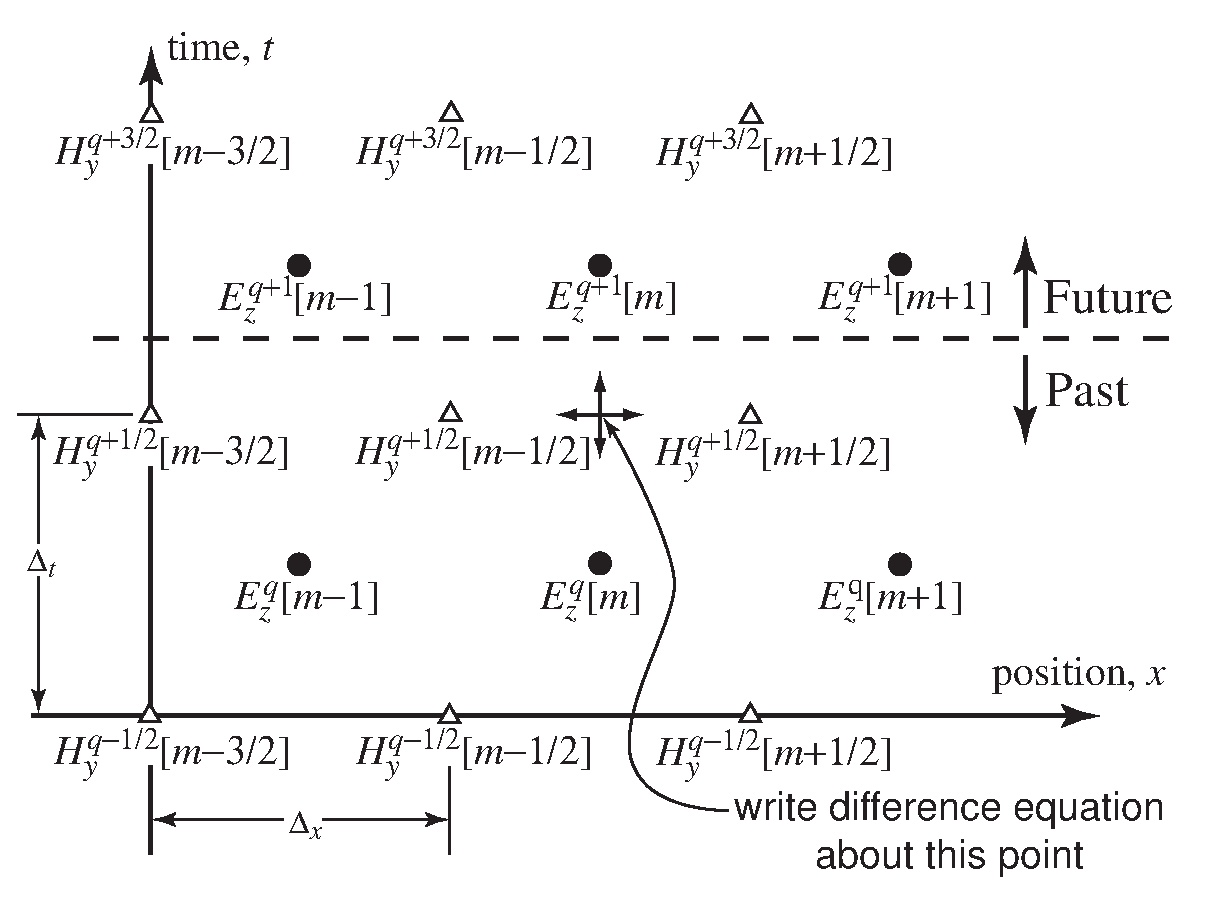
\epsfig{width=4.6in,file=Figures/Fdtd-intro/space-time-fdtd-new.eps}
  \end{center}
  \caption{Space-time after updating the magnetic field.  The dividing
  line between future and past values has moved forward a half
  temporal step.  The indicated point is where the difference equation
  is written to obtain an update equation for $E_z$.}
  \label{fig:spaceTimeUpdate}
\end{figure}
\begin{equation}
  \left.\epsilon
  \frac{\partial E_z}{\partial t}\right|_{m\Delx,(q+1/2)\Delt}
  =
  \left.\frac{\partial H_y}{\partial x}\right|_{m\Delx,(q+1/2)\Delt}.
\end{equation}
Replacing the temporal derivative on the left with a finite
difference involving $\fdtd{E_z}{m}{q+1}$ and $\fdtd{E_z}{m}{q}$
and replacing the spatial derivative on the right with a finite
difference involving $\fdtdh{H_y}{m+\half}{q+\half}$ and
$\fdtdh{H_y}{m-\half}{q+\half}$ yields
\begin{equation}
  \epsilon\frac{\fdtd{E_z}{m}{q+1} - \fdtd{E_z}{m}{q}}{\Delt} = 
  \frac{\fdtdh{H_y}{m+\half}{q+\half} - \fdtdh{H_y}{m-\half}{q+\half}}{\Delx}.
  \label{eq:ampereFdtd1D}
\end{equation}
Solving for $\fdtd{E_z}{m}{q+1}$ yields
\begin{equation}
  \fdtd{E_z}{m}{q+1} = \fdtd{E_z}{m}{q} + 
  \frac{\Delt}{\epsilon\Delx}
   \left(\fdtdh{H_y}{m+\half}{q+\half} - \fdtdh{H_y}{m-\half}{q+\half}\right).
  \label{eq:updateEz}
\end{equation}
Equation \refeq{eq:updateEz} is the update equation for the $E_z$
field.  The indices in this equation are generic so that the same
equation holds for every $E_z$ node.  Similar to the update equation for
the magnetic field, here we see that the future value of $E_z$ depends
on only its past value and the value of the neighboring magnetic
fields.
\index{update equation!one-dimensional|)}

After applying \refeq{eq:updateEz} to every electric-field node in the
grid, the dividing line between what is known and what is unknown
moves forward another one-half temporal step.  One is essentially back
to the situation depicted in Fig.\ \ref{fig:spaceTime}---the future
fields closest to the dividing line between the future and past are
magnetics fields.  They would be updated again, then the electric
fields would be updated, and so on.

It is often convenient to represent the update coefficients
$\Delt/\epsilon\Delx$ and $\Delt/\mu\Delx$ in terms of the ratio of
how far energy can propagate in a single temporal step to the spatial
step.  The maximum speed electromagnetic energy can travel is the
speed of light in free space $c=1/\sqrt{\epsilon_0\mu_0}$ and hence
the maximum distance energy can travel in one time step is $c\Delt$
(in all the remaining discussions the symbol $c$ will be reserved for
the speed of light in free space).  The ratio $c\Delt/\Delx$ is often
called the Courant number \index{Courant number!definition} which we
label $S_c$.  It plays an important role in determining the stability
of a simulation (hence the use of $S$) and will be considered further
later.  Letting $\mu=\mu_r\mu_0$ and $\epsilon=\epsilon_r\epsilon_0$,
the coefficients in \refeq{eq:updateEz} and \refeq{eq:updateHy} can be
written
\begin{eqnarray}
  \frac{1}{\epsilon} \frac{\Delt}{\Delx} \!&=&\!
    \frac{1}{\epsilon_r\epsilon_0}
    \frac{\sqrt{\epsilon_0\mu_0}}{\sqrt{\epsilon_0\mu_0}}
    \frac{\Delt}{\Delx} = 
    \frac{\sqrt{\epsilon_0\mu_0}}{\epsilon_r\epsilon_0}
    \frac{c\Delt}{\Delx} = 
    \frac{1}{\epsilon_r}
    \sqrt{\frac{\mu_0}{\epsilon_0}}
    \frac{c\Delt}{\Delx} = 
    \frac{\eta_0}{\epsilon_r}
    \frac{c\Delt}{\Delx} =
    \frac{\eta_0}{\epsilon_r} S_c
  \label{eq:coefEz} \\
  \frac{1}{\mu} \frac{\Delt}{\Delx} \!&=&\!
    \frac{1}{\mu_r\mu_0}
    \frac{\sqrt{\epsilon_0\mu_0}}{\sqrt{\epsilon_0\mu_0}}
    \frac{\Delt}{\Delx} = 
    \frac{\sqrt{\epsilon_0\mu_0}}{\mu_r\mu_0}
    \frac{c\Delt}{\Delx} = 
    \frac{1}{\mu_r}
    \sqrt{\frac{\epsilon_0}{\mu_0}}
    \frac{c\Delt}{\Delx} = 
    \frac{1}{\mu_r\eta_0}
    \frac{c\Delt}{\Delx} =
    \frac{1}{\mu_r\eta_0} S_c
    \label{eq:coefHy}
\end{eqnarray}
where $\eta_0=\sqrt{\mu_0/\epsilon_0}$ is the characteristic impedance
of free space.

In FDTD simulations there are restrictions on how large a temporal
step can be.  If it is too large, the algorithm produces unstable
results (i.e., the numbers obtained are completely meaningless and
generally tend quickly to infinity).  At this stage we will not
consider a rigorous analysis of stability.  However, thinking about
the way fields propagate in an FDTD grid, it seems logical that energy
should not be able to propagate any further than one spatial step for
each temporal step, i.e., $c\Delt\le\Delx$.  This is because in the
FDTD algorithm each node only affects its nearest neighbors.  In one
complete cycle of updating the fields, the furthest a disturbance could
propagate is one spatial step.  It turns out that the optimum ratio
for the Courant number (in terms of minimizing numeric errors)
is also the maximum ratio.  Hence, for the one-dimensional simulations
considered initially, we will use
\begin{equation}
  S_c = \frac{c\Delt}{\Delx} = 1.
\end{equation}

When first obtaining the update equations for the FDTD algorithm, it
is helpful to think in terms of space-time.  However, treating time as
an additional dimension can be awkward.  Thus, in most situations it
is more convenient to think in terms of a single spatial dimension
where the electric and magnetic fields are offset a half spatial step
from each other.  This is depicted in Fig.\
\ref{fig:fdtdOneD}.  The temporal offset between the electric and
magnetic field is always understood whether explicitly shown or not.
\begin{figure}
  \begin{center}
  \epsfig{width=5.0in,file=Figures/Fdtd-intro/space-fdtd-1d.eps}
  \end{center}
  \caption{A one-dimensional FDTD space showing the spatial offset
  between the magnetic and electric fields.}
  \label{fig:fdtdOneD}
\end{figure}


\section{Computer Implementation of a One-Dimensional\\ FDTD Simulation}

Our goal now is to translate the update equations \refeq{eq:updateHy}
and \refeq{eq:updateEz} into a usable computer program.  The first
step is to discard, at least to a certain extent, the
superscripts---time is a global parameter and will be recorded in a
single integer variable.  Time is not something about which each node
needs to be concerned.

Next, keep in mind that in most computer languages the equal sign is
used as ``the assignment operator.''  In C, the following is a
perfectly valid statement
\begin{verbatim}
  a = a+b;
\end{verbatim}
In the usual mathematical sense, this statement is only true if $b$
were zero.  However, to a computer this statement means take the value
of $b$, add it to the old value of $a$, and place the result back in
the variable $a$.  Essentially we are updating the value of $a$.  In C
this statement can be written more tersely as
\begin{verbatim}
  a += b;
\end{verbatim}

When writing a computer program to implement the FDTD algorithm, one
does not bother trying to construct a program that explicitly uses
offsets of one-half.  Nodes are stored in arrays and, as is standard
practice, individual array elements are specified with integer
indices.  Thus, the computer program (or, perhaps more correctly, the
{\em author} of the computer program) implicitly incorporates the fact
that electric and magnetic fields are offset while using only integer
indices to specify location.  As you will see, spatial location and
the array index will be virtually synonymous.

For example, assume two arrays, {\tt ez} and {\tt hy}, are
declared which will contain the $E_z$ and $H_y$ fields at 200 nodes
\begin{verbatim}
  double ez[200], hy[200], imp0=377.0;
\end{verbatim}
The variable {\tt imp0} is the characteristic impedance of free space
and will be used in the following discussion (it is initialized to a
value of $377.0$ in this declaration).  One should think of the
elements in the {\tt ez} and {\tt hy} arrays as being offset from
each other by a half spatial step even though the array values will be
accessed using an integer index.  

It is arbitrary whether one initially wishes to think of an {\tt ez}
array element as existing to the right or the left of an {\tt hy}
element with the same index (we assume ``left'' corresponds to
descreasing values of $x$ while ``right'' corresponds to increasing
values).  Here we will assume {\tt ez} nodes are to the left of {\tt
  hy} nodes with the same index.  This is illustrated in Fig.\
\ref{fig:oneDArrays} where {\tt ez[0]} is to the left of {\tt hy[0]},
{\tt ez[1]} is to the left of {\tt hy[1]}, and so on.  In general,
when a Courier font is used, e.g., {\tt hy[m]}, we are considering an
array and any offsets of one-half associated with that array are
implicitly understood.  When Times-Italic font is use, e.g.,
$\fdtdh{H_y}{m+\half}{q+\half}$ we are discussing the field itself and
offsets will be given explicitly.
\begin{figure}
  \begin{center}
  \epsfig{width=5.0in,file=Figures/Fdtd-intro/fdtd-1d-computer.eps}
  \end{center}
  \caption{A one-dimensional FDTD space showing the assumed spatial
  arrangement of the electric- and magnetic-field nodes in the arrays
  {\tt ez} and {\tt hy}.  Note that an electric-field node is assumed
  to exist to the left of the magnetic-field node with the same
  index.}  \label{fig:oneDArrays}
\end{figure}

Assuming a Courant number of unity ($S_c=1$), the node {\tt hy[1]}
could be updated with a statement such as
\begin{verbatim}
  hy[1] = hy[1] + (ez[2] - ez[1]) / imp0;
\end{verbatim}
In general, any magnetic-field node can be updated with
\begin{verbatim}
  hy[m] = hy[m] + (ez[m + 1] - ez[m]) / imp0;
\end{verbatim}
For the electric-field nodes, the update equation can be written
\begin{verbatim}
  ez[m] = ez[m] + (hy[m] - hy[m - 1]) * imp0;
\end{verbatim}
These two update equations, placed in appropriate loops, are the
engines that drive an FDTD simulation.  However, there are a few
obvious pieces missing from the puzzle before a useful simulation can
be performed.  These missing pieces include
\begin{enumerate}
\item Nodes at the end of the physical space do not have neighboring
  nodes to one side.  For example, there is no {\tt hy[-1]} node for
  the {\tt ez[0]} node to use in its update equation.  Similarly, if
  the arrays are declared with 200 element, there is no {\tt ez[200]}
  available for {\tt hy[199]} to use in its update equation (recall
  that the index of the last element in a C array is one less than the
  total number of elements---the array index represents the offset
  from the first element of the array).  Therefore a standard update
  equation cannot be used at these nodes.

\item Only a constant impedance is used so only a homogeneous medium
  can be modeled (in this case free space).

\item As of yet there is no energy present in the field.  If the
  fields are initially zero, they will remain zero forever.
\end{enumerate}

The first issue can be addressed using absorbing boundary conditions
(ABC's).  There are numerous implementations one can use.  In later
material we will be consider only a few of the more popular
techniques.

The second restriction can be removed by allowing the permittivity and
permeability to change from node to node.  However, in the interest of
simplicity, we will continue to use a constant impedance for a little
while longer.

The third problem can be overcome by initializing the fields to a
non-zero state.  However, this is cumbersome and typically not a good
approach.  Better solutions are to introduce energy via either a
hardwired source, an additive source, or a total-field/scattered-field
(TFSF) boundary.  We will consider implementation of each of these
approaches.

\section{Bare-Bones Simulation \label{sec:bareBones}}

Let us consider a simulation of a wave propagating in free space where 
there are 200 electric- and magnetic-field nodes.  The code is shown
in Program \ref{pro:1DbareBones}.
\begin{program}
{\tt 1DbareBones.c}: \index{1DbareBones.c@{\tt 1DbareBones.c}}
Bare-bones one-dimensional simulation with a hard
source. \label{pro:1DbareBones}
\codemiddle
\begin{lstlisting}
/* Bare-bones 1D FDTD simulation with a hard source. */

#include <stdio.h>
#include <math.h>

#define SIZE 200

int main()
{
  double ez[SIZE] = {0.}, hy[SIZE] = {0.}, imp0 = 377.0; /*@ \label{bareBonesA} @*/
  int qTime, maxTime = 250, mm;              /*@ \label{bareBonesB} @*/

  /* do time stepping */
  for (qTime = 0; qTime < maxTime; qTime++) {  /*@ \label{bareBonesC} @*/

    /* update magnetic field */
    for (mm = 0; mm < SIZE - 1; mm++)            /*@ \label{bareBonesD} @*/
      hy[mm] = hy[mm] + (ez[mm + 1] - ez[mm]) / imp0;

    /* update electric field */
    for (mm = 1; mm < SIZE; mm++)              /*@ \label{bareBonesE} @*/
      ez[mm] = ez[mm] + (hy[mm] - hy[mm - 1]) * imp0;

    /* hardwire a source node */
    ez[0] = exp(-(qTime - 30.) * (qTime - 30.) / 100.); /*@ \label{bareBonesF} @*/

    printf("%g\n", ez[50]); /*@ \label{bareBonesG} @*/
  } /* end of time-stepping */

  return 0;
}
\end{lstlisting}
\end{program}
In the declaration of the field arrays in line \ref{bareBonesA},
``{\tt=\{0.\}}'' has been added to ensure that these arrays are
initialized to zero.  (For larger arrays this is not an efficient
approach for initializing the arrays and we will address this fact
later.)  The variable {\tt qTime} is an integer counter that serves as
the temporal index or time step.  The total number of time steps in
the simulation is dictated by the variable {\tt maxTime} which is set
to $250$ in line \ref{bareBonesB} ($250$ was chosen arbitrarily---it
can be any value desired).

Time-stepping is accomplished with the for-loop that begins on line
\ref{bareBonesC}.  Embedded within this time-stepping loop are two
additional (spatial) loops---one to update the magnetic field and the
other to update the electric field.  The magnetic-field update loop
starting on line \ref{bareBonesD} excludes the last magnetic-field
node in the array, {\tt hy[199]}, since this node lacks one
neighboring electric field.  For now we will leave this node zero.
The electric-field update loop in line \ref{bareBonesE} starts with a
spatial index {\tt m} of $1$, i.e., it does not include {\tt ez[0]}
which is the first $E_z$ node in the grid.  The value of {\tt ez[0]}
is dictated by line \ref{bareBonesF} which is a Gaussian function that
will have a maximum value of unity when the time counter {\tt qTime}
is $30$.  The first time through the loop, when {\tt qTime} is zero,
{\tt ez[0]} will be set to $\exp(-9)\approx 1.2341\times 10^{-4}$
which is small relative to the maximum value of the source.  Line
\ref{bareBonesG} prints the value of {\tt ez[50]} to the screen, once
for each time step.  A plot of the output generated by this program is
shown in Fig.\
\ref{fig:bareBones}.
\begin{figure}
  \begin{center}
  \epsfig{width=4.6in,file=Code/Fdtd-intro/bare-bones-output200.eps}
  \end{center}
  \caption{Output generated by Program \ref{pro:1DbareBones}.}
  \label{fig:bareBones} 
\end{figure}

Note that the output is a Gaussian.  The excitation is introduced at
{\tt ez[0]} but the field is recorded at {\tt ez[50]}.  Because
$c\Delt=\Delx$ in this simulation (i.e., the Courant number is unity),
the field moves one spatial step for every time step.  The separation
between the source point and the observation point results in the
observed signal being delayed by $50$ time steps from what it was at
the source.  The source function has a peak at $30$ time steps but, as
can be seen from Fig.\ \ref{fig:bareBones}, the field at the
observation point is maximum at time step $80$.

Consider a slight modification to Program \ref{pro:1DbareBones} where
the simulation is run for $1000$ time steps instead of $250$ (i.e.,
{\tt maxTime} is set to $1000$ in line \ref{bareBonesB} instead of
$250$).  The output obtained in this case is shown in Fig.\
\ref{fig:bareBonesLong}.
\begin{figure}
  \begin{center}
  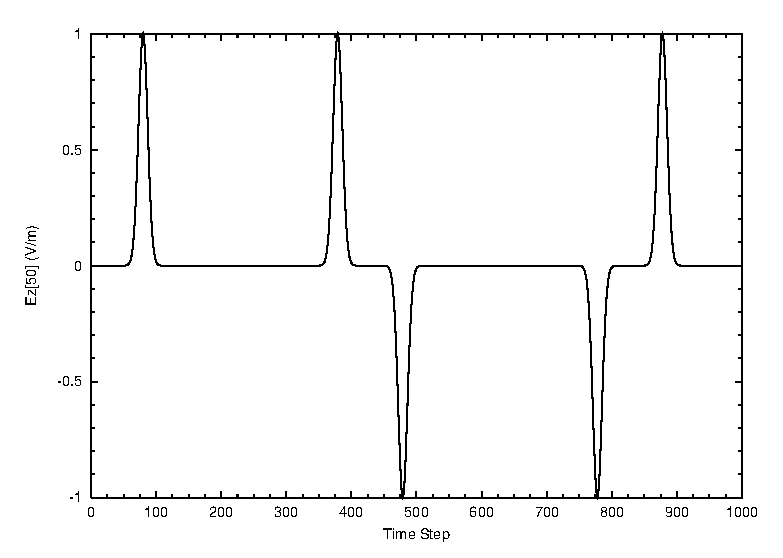
\epsfig{width=4.6in,file=Code/Fdtd-intro/bare-bones-output1000.eps}
  \end{center}
  \caption{Output generated by Program \ref{pro:1DbareBones} but with
  {\tt maxTime} set to $1000$.}
  \label{fig:bareBonesLong} 
\end{figure}
Why are there multiple peaks here and why are they both positive and
negative?

The last magnetic-field node in the grid is initially zero and remains
zero throughout the simulation.  When the field encounters this node
it essentially see a perfect magnetic conductor (PMC).  To satisfy the
boundary condition at this node, i.e., that the total magnetic field
go to zero, a reflected wave is created which reverses the sign of the
magnetic field but preserves the sign of the electric field.  This
phenomenon is considered in more detail in the next section.  The
second peak in Fig.\ \ref{fig:bareBonesLong} is this reflected wave.
The reflected wave continues to travel in the negative direction until
it encounters the first electric-field node {\tt ez[0]}.  This node
has its value set by the source function and is oblivious to what is
happening in the interior of the grid.  In this particular case, by
the time the reflected field reaches the left end of the grid, the
source function has essentially gone to zero and nothing is going to
change that.  Thus the node {\tt ez[0]} behaves like a perfect
electric conductor (PEC).  To satisfy the boundary conditions at this
node, the wave is again reflected, but this time the electric field
changes sign while the sign of the magnetic field is preserved.  In
this way the field which was introduced into the grid continues to
bounce back and forth until the simulation is terminated.  The
simulation is of a resonator with one PMC wall and one PEC wall.
(Note that the boundary condition at {\tt ez[0]} is the same whether
or not the source function has gone to zero.  Any incoming field
cannot change the value at {\tt ez[0]} and hence a reflected wave must
be generated which has equal magnitude but opposite sign from the
incoming field.)

%%%%%%%%%%%%%%%%%%%%%%%%%%%%%%%%%%%%%%%%%%%%%%%%%%%%%%%%%%%%%%%%%%%%%%%%%
\section{PMC Boundary in One Dimension \label{sec:pmcBoundary}} 

In Program \ref{pro:1DbareBones} one side of the grid (the ``right
side'') is terminated by a magnetic field which is always zero.  It
was observed that this node acts as a perfect magnetic conductor (PMC)
which produces a reflected wave where the electric field is not
inverted while the magnetic field is inverted.  To understand fully
why this is the case, let us consider the right side of a
one-dimensional domain where $200$ electric- and magnetic-field nodes
are used to model free space.  Assume the Courant number is unity and
the impedance of free space is $377$.  The last node in the grid is
{\tt hy[199]} and it will always remain zero.  The other nodes in the
grid are updated using, in C notation:
\begin{eqnarray}
  \mbox{\tt\ \ \ \ ez[m] = ez[m] + (hy[m] - hy[m - 1]) * 377;} \label{eq:ezUpdateC}\\
  \mbox{\tt\ \ \ \ hy[m] = hy[m] + (ez[m + 1] - ez[m]) / 377;} \label{eq:hyUpdateC}
\end{eqnarray}
Assume that a Dirac delta pulse, i.e., a unit amplitude pulse existing
at a single electric-field node in space-time, is nearing the end of
the grid.  Table \ref{tab:pmcBoundary} shows the fields at progressive
time-steps starting at a time $q$ when the pulse has reached node {\tt
ez[198]}.

\renewcommand{\multirowsetup}{\centering}
\newlength{\LL}\settowidth{\LL}{time}
\begin{table}
\begin{center}
\begin{tabular}{cl|cccccc}
\multirow{12}{\LL}{time\\step}& & \multicolumn{6}{c}{node} \\
&
& {\tt ez[197]} &{\tt hy[197]} &{\tt ez[198]}&
  {\tt hy[198]} &{\tt ez[199]} &{\tt hy[199]}\\ \hline
& $q-1/2$&       &$-1/377$ &     &$0$      &       &$0$\\
& $q$    &  $0$  &         &$1$  &         &$0$    &\\ \cline{2-8}
& $q+1/2$&       &$0$      &     &$-1/377$ &       &$0$\\
& $q+1$  &  $0$  &         &$0$  &         &$1$    &\\ \cline{2-8}
& $q+3/2$&       &$0$      &     &$0$      &       &$0$\\
& $q+2$  &  $0$  &         &$0$  &         &$1$    &\\ \cline{2-8}
& $q+5/2$&       &$0$      &     &$1/377$  &       &$0$\\
& $q+3$  &  $0$  &         &$1$  &         &$0$    &\\ \cline{2-8}
& $q+5/2$&       &$1/377$  &     &$0$      &       &$0$ \\
& $q+4$  &  $1$  &         &$0$  &         &$0$    &
\end{tabular}
\end{center}
\caption{Electric- and magnetic-field nodes at the ``end'' of arrays
 which have 200 elements, i.e., the last node is {\tt hy[199]} which is
 always set to zero.  A pulse of unit amplitude is propagating to the
 right and has arrived at {\tt ez[198]} at time-step $q$.  Time is
 advancing as one reads down the columns.}
\label{tab:pmcBoundary}
\end{table}

At time $q$ node {\tt ez[198]} is unity while {\tt hy[197]} was set to
$-1/377$ at the previous update of the magnetic fields.  When the
magnetic fields are updated at time $q+1/2$ the update equation
\refeq{eq:hyUpdateC} dictates that {\tt hy[197]} be set to zero (the
``old'' value of the magnetic field cancels the contribution from the
electric field).  Meanwhile, {\tt hy[198]} becomes $-1/377$.  All
other magnetic-field nodes will be zero.

Updating the electric field at time-step $q+1$ results in {\tt
ez[198]} being set to zero while {\tt ez[199]} is set to one---the
pulse advances one spatial step to the right.  If the normal update
equation could be used at node {\tt hy[199]}, at time $q+3/2$ it would
be set to $-1/377$.  However, because there is no neighboring electric
field to the right of {\tt hy[199]}, the update equation cannot be
used and, lacking an alternative way of calculating its value, {\tt
hy[199]} is left as zero.  Thus at time $q+3/2$ {\em all} the
magnetic-field nodes in the grid are zero.

When the electric field is updated at time $q+2$ essentially nothing
happens.  The electric fields are updated from their old values and
the difference of surrounding magnetic fields.  However all magnetic
fields are zero.  Thus the new electric field is the same as the old
electric field.

At time $q+5/2$ the unit pulse which exists at {\tt ez[199]} causes
{\tt hy[198]} to become $1/377$ which is the negative of what it was two
times steps ago.  From this time forward, the pulse propagates back to
the left with the electric field maintaining unit amplitude.

This discussion is for a single pulse, but any incident field could be
treated as a string of pulses and then one would merely have to
superimpose their values.  This dicussion further supposes the Courant
number is unity.  When the Courant number is not unity the termination
of the grid still behaves as a PMC wall, but the pulse will not
propagate without distortion (it suffers dispersion because of the
properties of the grid itself as will be discussed in more detail in
Sec.\ \ref{sec:gridDispersion}).

If the grid were terminated on an electric-field node which was
always set to zero, that node would behave as a perfect electric
conductor.  In that case the reflected electric field would have the
opposite sign from the incident field while the magnetic field would
preserve its sign.  This is what happens to any field incident on the
left side of the grid in Program \ref{pro:1DbareBones}.

\section{Snapshots of the Field}

In Program \ref{pro:1DbareBones} the field at a single point is
recorded to a file.  Alternatively, it is often useful to view the
fields over the entire computational domain at a single instant of
time, i.e., take a ``snapshot'' that shows the field throughout space.
Here we describe one way in which this can be conveniently implemented
in C.

The approach adopted here will open a separate file for each snapshot.
Each file will have a common base name, then a dot, and then a
sequence number which will be called the frame number.  So, for
example, the files might be called {\tt sim.0}, {\tt sim.1}, {\tt
sim.2}, and so on.  To accomplish this, the fragments shown in
Fragments \ref{frag:snapshot} and \ref{frag:snapshotI} would be added to a
program (such as Program \ref{pro:1DbareBones}).
\begin{fragment}
  Declaration of variables associated with taking snapshots.  The base
  name is stored in the character array {\tt basename} and the
  complete file name for each frame is stored in {\tt filename}.  Here
  the base name is initialized to {\tt sim} but, if desired, the user
  could be prompted for the base name.  The integer {\tt frame} is the
  frame number for each snapshot and is initialized to
  zero. \label{frag:snapshot}
  \codemiddle
\begin{lstlisting}
  char basename[80] = "sim", filename[100];
  int frame = 0;
  FILE *snapshot;
\end{lstlisting}
\end{fragment}
\begin{fragment}
  Code to generate the snapshots.  This would be placed inside the
  time-stepping loop.  The initial if statement ensures the electric
  field is recorded every tenth time-step.\label{frag:snapshotI}
  \codemiddle
\begin{lstlisting}
    /* write snapshot if time-step is a multiple of 10 */
    if (qTime % 10 == 0) {                       /*@ \label{fragSnapA} @*/
      /* construct complete file name and increment frame counter */
      sprintf(filename, "%s.%d", basename, frame++); /*@ \label{fragSnapB} @*/

      /* open file */
      snapshot = fopen(filename, "w");  /*@ \label{fragSnapC} @*/

      /* write data to file */
      for (mm = 0; mm < SIZE; mm++)     /*@ \label{fragSnapD} @*/
        fprintf(snapshot, "%g\n", ez[mm]);

      /* close file */
      fclose(snapshot);                 /*@ \label{fragSnapE} @*/
    }
\end{lstlisting}
\end{fragment}

In Fragment \ref{frag:snapshot} the base name is initialized to {\tt
  sim} but the user could be prompted for this.  The integer variable
{\tt frame} is the frame (or snapshot) counter that will be
incremented each time a snapshot is taken.  It is initialized to zero.
The file pointer {\tt snapshot} is used for the output files.

The code shown in Fragment \ref{frag:snapshotI} would be placed inside
the time-stepping loop of Program \ref{pro:1DbareBones}.  Line
\ref{fragSnapA} checks, using the modulo operator ({\tt \%}) if the
time step is a multiple of $10$.  ($10$ was chosen somewhat
arbitrarily.  If snapshots were desired more frequently, a smaller
value would be used.  If snapshots were desired less frequently, a
larger value would be used.)  If the time step is a multiple of $10$,
the complete output-file name is constructed in line \ref{fragSnapB}
by writing the file name to the string variable {\tt filename}.
(Since zero is a multiple of $10$, the first snapshot that is taken
corresponds to the fields at time zero.  This data would be written to
the file {\tt sim.0}.  Note that in Line \ref{fragSnapB} the frame
number is incremented each time a file name is created.  The file is
opened in line \ref{fragSnapC} and the data is written using the loop
starting in line \ref{fragSnapD}.  Finally, the file is closed in line
\ref{fragSnapE}.

Fig.\ \ref{fig:snapshots} shows the snapshots of the field at time
steps $20$, $30$, and $40$ using essentially the same code as Program
\ref{pro:1DbareBones}---the only difference being the addition of the
code to take the snapshots.  The corresponding files are {\tt sim.2},
{\tt sim.3}, and {\tt sim.4}.  In these snapshots the field can be
seen entering the computational domain from the left and propagating
to the right.

\begin{figure}
  \begin{center}
  \epsfig{width=3.5in,file=Code/Fdtd-intro/snapshot1.eps}
  \epsfig{width=3.5in,file=Code/Fdtd-intro/snapshot2.eps}
  \epsfig{width=3.5in,file=Code/Fdtd-intro/snapshot3.eps}
\end{center} \caption{Snapshots taken at time-steps $20$, $30$, and
  $40$ of the $E_z$ field generated by Program \ref{pro:1DbareBones}.
  The field is seen to be propagating away from the hardwired source
  at the left end of the grid.}  \label{fig:snapshots}
\end{figure}

\section{Additive Source \label{sec:additive}}

Hardwiring the source, as was done in Program \ref{pro:1DbareBones},
has the severe shortcoming that no energy can pass through the source
node.  This problem can be rectified by using an additive source.
Consider Ampere's law with the current density term:
\begin{equation}
  \nabla\times\Hvec = \Jvec + 
                      \epsilon\frac{\partial \Evec}{\partial t}.
  \label{eq:ampereWithCurrent}
\end{equation}
The current density $\Jvec$ can represent both the conduction current
due to flow of charge in a material under the influence of the
electric field, i.e., current given by $\sigma\Evec$, as well as the
current associated with any source, i.e., an ``impressed current.''
At this point we are just interested in the source aspect of $\Jvec$
and will return to the issue of finite conductivity in Sec.\
\ref{sec:loss} and Sec.\ \ref{sec:conductivity}.  Rearranging
\refeq{eq:ampereWithCurrent} slightly yields
\begin{equation}
  \frac{\partial \Evec}{\partial t} =
     \frac{1}{\epsilon} \nabla\times\Hvec - \frac{1}{\epsilon}\Jvec.
  \label{eq:ampereTweak}
\end{equation}
This equation gives the temporal derivative of the electric field in
terms of the spatial derivative of the magnetic field---which is as
before---and an additional term which can be thought of as the forcing
function for the system.  This current can be specified to be whatever
is desired.

To translate \refeq{eq:ampereTweak} into a form suitable for the FDTD
algorithm, the spatial derivatives are again expressed in terms of
finite differences and then one solves for the future fields in terms
of past fields.  Recall that for Ampere's law, the update equation for
$\fdtd{E_z}{m}{q}$ was obtained by applying finite differences at the
space-time point $(m\Delx,(q+1/2)\Delt)$.  Going through the exact
same procedure but adding the source term yields
\begin{equation}
  \fdtd{E_z}{m}{q+1} = \fdtd{E_z}{m}{q} + 
  \frac{\Delt}{\epsilon\Delx}
   \left(\fdtdh{H_y}{m+\half}{q+\half} - \fdtdh{H_y}{m-\half}{q+\half}\right)
  - \frac{\Delt}{\epsilon}\fdtd{J_z}{m}{q+\half}.
  \label{eq:updateEzSource}
\end{equation}
The source current could potentially be distributed over a number of
nodes, but for the sake of introducing energy to the grid, it suffices
to apply it to a single node.

In order to preserve the original update equation (which is sometimes
handy when writing loops), \refeq{eq:updateEzSource} can be separated
into two steps: first the usual update is applied and then the source
term is added.  For example:
\begin{eqnarray}
  \fdtd{E_z}{m}{q+1} &=& \fdtd{E_z}{m}{q} + \frac{\Delt}{\epsilon\Delx}
    \left(\fdtdh{H_y}{m+\half}{q+\half} - \fdtdh{H_y}{m-\half}{q+\half}\right) \\
  \fdtd{E_z}{m}{q+1} &=& \fdtd{E_z}{m}{q+1} -
    \frac{\Delt}{\epsilon}\fdtd{J_z}{m}{q+\half}. \label{eq:addCurrent1D}
\end{eqnarray}
In practice the source current might only exist at a single node in
the 1D grid (as will be the case in the examples to come).  Thus,
\refeq{eq:addCurrent1D} would be applied only at the node where the
source current is non-zero.

Generally the amplitude and the sign of the source function are not a
concern.  When calculating things such as the scattering cross-section
or the reflection coefficient, one always normalizes by the incident
field.  Therefore we do not need to specify explicitly the value of
$\Delt/\epsilon$ in \refeq{eq:addCurrent1D}---it suffices to merely
treat this coefficient as being contained in the source function
itself.

A program that implements an additive source and takes snapshots of
the electric field is shown in Program \ref{pro:1Dadditive}.  The
changes from Program \ref{pro:1DbareBones} are shown in bold.  The
source function is exactly the same as before except now, instead of
setting the value of {\tt ez[0]} to the value of this function, the
source function is added to {\tt ez[50]}.  The source is introduced in
line \ref{1DadditiveE} and the update equations are unchanged from
before.  (Note that in this chapter the programs will be somewhat
verbose, simplistic, and repetitive.  Once we are comfortable with the
FDTD algorithm we will pay more attention to better coding practices.)
\begin{program}
{\tt 1Dadditive.c}: \index{1Dadditive.c@{\tt 1Dadditive.c}}
One-dimensional FDTD program with an additive
source. \label{pro:1Dadditive} 
\codemiddle
\begin{lstlisting}
/* 1D FDTD simulation with an additive source. */

#include <stdio.h>
#include <math.h>

#define SIZE 200

int main()
{
  double ez[SIZE] = {0.}, hy[SIZE] = {0.}, imp0 = 377.0;
  int qTime, maxTime = 200, mm;
/*b*/
  char basename[80] = "sim", filename[100];
  int frame = 0;
  FILE *snapshot;
/*n*/
  /* do time stepping */
  for (qTime = 0; qTime < maxTime; qTime++) {
                                                  /*@ \label{1DadditiveA} @*/
    /* update magnetic field */                   /*@ \label{1DadditiveB} @*/
    for (mm = 0; mm < SIZE - 1; mm++)
      hy[mm] = hy[mm] + (ez[mm + 1] - ez[mm]) / imp0;
                                                  /*@ \label{1DadditiveC} @*/
    /* update electric field */                   /*@ \label{1DadditiveD} @*/
    for (mm = 1; mm < SIZE; mm++)
      ez[mm] = ez[mm] + (hy[mm] - hy[mm - 1]) * imp0;
/*b*/
    /* use additive source at node 50 */
    ez[50] += exp(-(qTime - 30.) * (qTime - 30.) / 100.); /*@ \label{1DadditiveE} @*/

    /* write snapshot if time a multiple of 10 */
    if (qTime % 10 == 0) {
      sprintf(filename, "%s.%d", basename, frame++);
      snapshot=fopen(filename, "w");
      for (mm = 0; mm < SIZE; mm++)
        fprintf(snapshot, "%g\n", ez[mm]);
      fclose(snapshot);
    }/*n*/
  } /* end of time-stepping */

  return 0;
}
\end{lstlisting}
\end{program}

Snapshots of $E_z$ taken at time-steps $20$, $30$, and $40$ are shown
in Fig.\ \ref{fig:additive}.  Note that the field originates from node
$50$ and that it propagates to either side of this node.  Also notice
that the peak amplitude is half of what it was when the source
function was implemented as a hardwired source.
\begin{figure}
  \begin{center}
  \epsfig{width=3.5in,file=Code/Fdtd-intro/additive1.eps}
  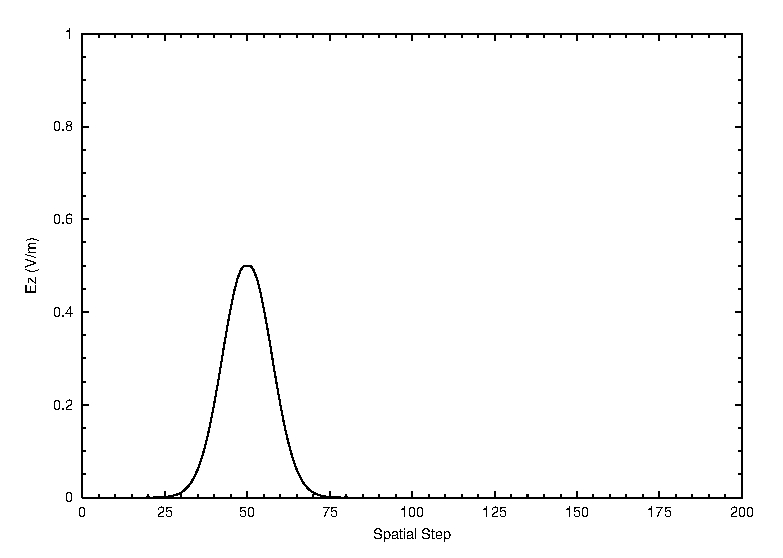
\epsfig{width=3.5in,file=Code/Fdtd-intro/additive2.eps}
  \epsfig{width=3.5in,file=Code/Fdtd-intro/additive3.eps}
  \end{center}
  \caption{Snapshots taken at time-steps $20$, $30$, and $40$ of the
    $E_z$ field generated by Program \ref{pro:1Dadditive}.  An
    additive source is applied to node $50$ and the field is seen to
    propagate away from it to either side.}
  \label{fig:additive} 
\end{figure}

As something of an aside, in Program \ref{pro:1Dadditive} note that
the code that takes a snapshot of the electric field was placed in the
time-stepping but after the update equation.  Thus one might ask: do
the contents of snapshot file {\tt sim.0} contain the fields at time
zero or at time one?  And, do the other snapshots correspond to times
that multiples of $10$ or do the correspond to one plus a multiple of
$10$?  In nearly all practical cases it won't matter.  The precise
location of $t=0$ is rather arbitrary.  So, when looking at the
snapshots it is usually sufficient to know that the sequence of
snapshots start ``at the beginning of the simulation'' and then are
taken every $10$ time steps.  However, if one wants to be more precise
about this, absolute time is usually dictated by the source function.
Now, think in terms of the hard-source implementation rather than the
additive source.  We have implemented a Gaussian source that has a
peak amplitude at time-step $30$.  The way the code is written here,
with the source being applied after the update equation and then the
snapshot being taken last, we would see the peak at the source node in
frame {\tt sim.1}.  In other words the snapshots do indeed correspond
to times that are multiples of $10$.  So, in some sense the electric
fields start at a time step of $-1$.  The very first update
loop takes them up to time step $0$, and then the source function is
applied to set the field at the source node at time-step $0$.  {\em
  However}, this is truly a minor point and we will not worry about it
in subsequent discussions.  Whether the code that introduces the
source appears before or after the update loop and whether the code
that generates output appears before or after the update loop, often
doesn't matter---the important thing is generally just that these
things are included in the time-stepping loop.

\section{Terminating the Grid \label{sec:terminate}}

In most instances one is interested in modeling a problem which exists
in an open domain, i.e., an infinite space.  This is true even when
the specific region of interest, say the region where a scatterer is
present, may be small.  That scatterer is in an unbounded space.  Thus
far the code we have written is only suitable for modeling a resonator
since the nodes at the ends of the grid reflect any field incident
upon them.  We now wish to rectify this shortcoming.  Absorbing
boundary conditions (ABC's) will be used so that the grid, which will
contain only a finite number of nodes, can behave as if it were
infinite.  In one dimension, when operating at the Courant limit of
one, an exact ABC can be realized.  Unfortunately in higher
dimensions, or even in one dimension when not operating at the Courant
limit, ABC's are only approximate.  The better the ABC, the less
energy it reflects back into the interior of the grid.

Before implementing an ABC, let us again consider the code shown in
Program \ref{pro:1Dadditive} but with the maximum number of time steps
set to $450$.  With the FDTD method, the more ways in which the field
can be visualized, the better.  Watching the field propagate in the
time-domain can provide insights into the behavior of a system.
Additionally, visualization of the propagation of the fields can be an
invaluable aid when debugging FDTD code.  Animations of the field are
especially useful and different display strategies will be discussed
later.  

Since we cannot include an animation here, we will use a ``waterfall
plot'' \index{waterfall plot} of the electric field in the
one-dimensional domain.  A waterfall plot is a collection of standard
``$x$ vs.\ $y$'' plots where each plot is offset slightly from the
next (a direct vertical offset will be used here).  This can be
thought of as stacking all the frames of an animation, one above the
next.

Figure \ref{fig:waterfall} shows the waterfall plot corresponding to
the output from Program \ref{pro:1Dadditive} (with a {\tt maxTime} of
450).
\begin{figure}
  \begin{center}
  \epsfig{width=4.6in,file=Code/Fdtd-intro/waterfall.eps}
  \end{center}
  \caption{Waterfall plot of the electric field produced by Program
    \ref{pro:1Dadditive}.  The computational domain has $200$ nodes
    with a PEC boundary on the left and a PMC boundary on the right.
    The vertical axis gives the frame number.  Snapshots, i.e.,
    frames, were recorded every 10 time steps.}
  \label{fig:waterfall} 
\end{figure}
Each line represents a snapshot of the field throughout the
computational domain.  One can see that electric field starts to
propagate away from the source which is at node $50$.  The curve/line
corresponding to $5$ on the vertical axis is the data from the sixth
frame (i.e., {\tt sim.5}).  Since the frames are recorded every ten
time-steps, since {\tt sim.0} corresponds to the field at time zero,
this line shows the field at the fiftieth time-step.  This line has
two peaks.  One is traveling to the left and the other to the right.
Once the left-going field encounters the end of the grid at node zero,
it is both reflected and inverted.  It then travels to the right as
time progresses.  The peak which originally travels to the right from
the source encounters the right end of the grid around frame (or
curve) 17.  In this case, with the PMC boundary that exists there, the
electric field is not inverted---instead, the magnetic field, which is
not plotted, is inverted.  A reflected wave then propagates back to
the left.  The field propagates back and forth, inverting its sign at
the left boundary and preserving its sign at the right boundary, until
the simulation is halted.  The Matlab code that was used to generate
this waterfall plot is given in Appendix \ref{ap:waterfall}.
Additionally, Appendix \ref{ap:waterfall} provides Matlab code that
can be used to animate snapshots of a one-dimensional domain.

Returning to the issue of grid termination, when the Courant number is
unity, the distance the wave travels in one temporal step is equal to
one spatial step, i.e., $c\Delt = \Delx$.  We are interested in
modeling an open domain where there is no energy entering the grid
``from the outside.''  Therefore, for node {\tt ez[0]}, its updated
value should just be the previous value that existed at {\tt ez[1]}.
Since no energy is entering the grid from the left, the field at {\tt
ez[1]} must be propagating solely to the left.  At the next time step
the value that was at {\tt ez[1]} should now appear at {\tt ez[0]}.
Similar arguments hold at the other end of the grid.  The updated
value of {\tt hy[199]} should be the previous value of {\tt hy[198]}.

Thus, a simple ABC can be realized by adding the following line to
Program \ref{pro:1Dadditive} between lines \ref{1DadditiveC} and
\ref{1DadditiveD}
\begin{verbatim}
  ez[0] = ez[1];
\end{verbatim}
Similarly, the following line would be added between lines
\ref{1DadditiveA} and \ref{1DadditiveB}
\begin{verbatim}
  hy[SIZE-1] = hy[SIZE-2];
\end{verbatim}
The waterfall plot which is obtained for the electric field after
making these changes is shown in Fig.\ \ref{fig:waterfallABC}.
\begin{figure}
  \begin{center}
  \epsfig{width=4.6in,file=Code/Fdtd-intro/waterfall-abc.eps}
  \end{center}
  \caption{Waterfall plot of the electric field using the same
    computational domain as Fig.\ \ref{fig:waterfall} except a simple
    ABC has been used to terminate the grid.  Note that the field
    propagates from the additive source at node 50 and merely
    disappears when it reaches either end of the grid.}
  \label{fig:waterfallABC}
\end{figure}
Note that the reflected fields are no longer present.  The left- and
right-going pulses reach the end of the grid and then disappear as if
they have continued to propagate off to infinity.  (However, there is
still some persistent field that lingers throughout the grid.  This
field is small---about five orders of magnitude smaller than the peak
when using single precision---and is a consequence of finite
precision.  These small fields are not visible on the scale of the
plot and are not of much practical concern since typically other
sources of error will be far larger.)

As mentioned previously, this simple ABC only works in limited
situations.  However, the basic premise is employed in many of the
more complicated ABC's: the future value of the field at the end of the
grid depends on some combination of the past and interior fields.  We
will return to this topic in Chap.\ \ref{chap:abc}.

\section{Total-Field/Scattered-Field Boundary \label{sec:tfsf}}

Note that {\em any} function $f(\xi)$ which is twice differentiable is
a solution to the wave equation.  In one dimension all that is
required is that the argument $\xi$ be replaced by $t\pm x/c$.  A
proof was given in Sec.\ \ref{sec:waveEq}.  Thus far the excitation of
the FDTD grids has occurred at a point---either the hardwired source
at the left end of the grid, as shown in Program
\ref{pro:1DbareBones}, or the additive source at node $50$, as shown
in Program \ref{pro:1Dadditive}.  Now our goal is to construct a
source such that the excitation only propagates in one direction,
i.e., the source introduces an incident field that is propagating to
the right (the positive $x$ direction).  We will accomplish this using
what is known as a total-field/scattered-field (TFSF) boundary.

We start by specifying the incident field as a function of space and
time.  A Gaussian pulse has been used for the excitation in the
previous examples.  A Gaussian can still be used to specify the
excitation, but to obtain a wave propagating to the right, the
argument should be $t-x/c$ instead of merely $t$.  Previously the
source was given by
\begin{equation}
  f(t) = f(q\Delt)
       = e^{-\left(\frac{q\Delt - 30 \Delt}{10 \Delt}\right)^2} =
         e^{-\left(\frac{q - 30}{10}\right)^2} = f[q]
  \label{eq:sourceFunc}
\end{equation}
where $30\Delt$ is a delay and the term in the denominator of the
exponent ($10 \Delt$) controls the width of the pulse.  Note that the
time-step width $\Delt$ can be canceled from the numerator and
denominator of the exponent.

For the propagating incident field, $t$ in \refeq{eq:sourceFunc} is
replaced with $t-x/c$.  In discretized space-time this argument is
given by
\begin{equation}
  t-\frac{x}{c} = q\Delt-\frac{m\Delx}{c} =
  \left(q-\frac{m\Delx}{c\Delt}\right)\Delt
  = \left(q-m\right)\Delt
\end{equation}
where the assumption that the Courant number $c\Delt/\Delx$ is unity
has been used to write the last equality.  This expression can now be
used for the argument in the previous source function to obtain a
propagating wave which we will identify as $\Einc$
\begin{equation}
  \Einc[m,q]
       = e^{-\left(\frac{(q-m)\Delt - 30 \Delt}{10 \Delt}\right)^2}
       = e^{-\left(\frac{(q-m) - 30}{10}\right)^2}
\end{equation}
This equation essentially assumes that the origin, i.e., the point
$x=0$, corresponds to the index ${\mbox{\tt m}}=0$.  However, the
origin can be shifted to a different point and this fact will be
exploited later.  Keep in mind that there is nothing that dictates
that we must always think of the origin as corresponding to the
left-most point in the grid.

The corresponding magnetic field is obtained by dividing the electric
field by the characteristic impedance.  Additionally, to ensure that
$\Eincvec\times\Hincvec$ points in the desired direction of travel,
the magnetic field must be negative, i.e.,
\begin{equation}
  \Hinc[m,q] = -\sqrt{\frac{\epsilon}{\mu}}\Einc[m,q]
             = -\frac{1}{\eta}
                 e^{-\left(\frac{(q-m) - 30}{10}\right)^2}
\end{equation}
where $\eta=\sqrt{\mu/\epsilon}$ is the characteristic impedance of the
medium.  Note that the arguments do not need to be integers.  If one
needs to calculate the magnetic field at the position $m-1/2$ and time
$q-1/2$, these are perfectly legitimate arguments.

In the total-field/scattered-field (TFSF) formulation, the
computational domain is divided into two regions: (1) the total-field
region which contains the incident field plus any scattered field and
(2) the scattered-field region which contains only scattered field.
The incident field is introduced on an fictitious seam, or boundary,
between the total-field and the scattered-field regions.  The location
of this boundary is somewhat arbitrary, but it is typically placed so
that any scatterers are contained in the total-field region.

When updating the fields, the update equations must be consistent.
This is to say only scattered fields should be used to update a node
in the scattered-field region and only total fields should be used to
update a node in the total-field region.  Figure \ref{fig:tfsf} shows
a one-dimensional grid where the TFSF boundary is assumed to exist
between nodes $\fdtd{H_y}{49+\half}{}$ and $\fdtd{E_z}{50}{}$ (in
Fig.\ \ref{fig:tfsf} the nodes are shown in the computer-array form
with integer indices).  The node $\fdtd{H_y}{49+\half}{}$ is
equivalent to $\fdtd{H_y}{50-\half}{}$ and will be written using the
latter form in the following discussion.  Note that no matter where
the boundary is placed, there will only be two nodes adjacent to the
boundary---one electric-field node and one magnetic-field node.
Furthermore, although the location of this boundary is arbitrary, once
its location is selected, it is fixed throughout the simulation.
\begin{figure}
  \begin{center}
  \epsfig{width=5.0in,file=Figures/Fdtd-intro/fdtd-1d-tfsf.eps}
  \end{center}
  \caption{Portion of the one-dimensional arrays in the vicinity of a
  total-field/scattered-field boundary.  Scattered field 
  exists to the left of the boundary and total field exists
  to the right.  Note that node {\tt hy[49]} has an index of $49$ in a
  computer program but corresponds logically to
  the location $(49+\half)\Delx$ or, equivalently, $(50-\half)\Delx$.
  \label{fig:tfsf} }
\end{figure}
Defining the scattered-field region to be to the left of the boundary
and the total-field region to be to the right, we see that {\tt
hy[49]} is the last node in the scattered-field region while {\tt
ez[50]} is the first node in the total-field region.

When updating the nodes adjacent to the boundary, there is a problem,
i.e., an inconsistency, in that a neighbor to one side is not the same
type of field as the field being updated.  This is to say that a
total-field node will depend on a scattered-field node and,
conversely, a scattered-field node will depend on a total-field node.
The solution to this problem actually provides the way in which fields
are introduced into the grid using the TFSF boundary.

Consider the usual update equation of the electric field at location
$m=50$ which was given in \refeq{eq:updateEz} and is repeated below
\begin{equation}
  \overbrace{\fdtd{E_z}{50}{q+1}}^{\mbox{\scriptsize tot}}
  =
  \overbrace{\fdtd{E_z}{50}{q}}^{\mbox{\scriptsize tot}} + 
  \frac{\Delt}{\epsilon\Delx}
   \left(
  \overbrace{\fdtdh{H_y}{50+\half}{q+\half}}^{\mbox{\scriptsize tot}} -
  \overbrace{\fdtdh{H_y}{50-\half}{q+\half}}^{\mbox{\scriptsize scat}}
  \right).
  \label{eq:updateEzTFSF}
\end{equation}
We have assumed the TFSF boundary is between $\fdtd{E_z}{50}{q+1}$
and $\fdtdh{H_y}{50-\half}{q+\half}$ and the labels above the individual
components indicate if the field is in the total-field region or the
scattered-field region.  We see that $\fdtd{E_z}{50}{q+1}$ and
$\fdtdh{H_y}{50+\half}{q+\half}$ are total-field nodes but
$\fdtdh{H_y}{50-\half}{q+\half}$ is a scattered-field node---it lacks
the incident field.  This can be fixed by adding the incident field to
$\fdtdh{H_y}{50-\half}{q+\half}$ in
\refeq{eq:updateEzTFSF}.  This added field must correspond to the
magnetic field which exists at location $50-1/2$ and time step
$q+1/2$.  Thus, a consistent update equation for $\fdtd{E_z}{50}{q+1}$
which only involves total fields is
\begin{eqnarray}
  \overbrace{\fdtd{E_z}{50}{q+1}}^{\mbox{\scriptsize tot}} &=&
  \overbrace{\fdtd{E_z}{50}{q}}^{\mbox{\scriptsize tot}} + {} \\
  &&\frac{\Delt}{\epsilon\Delx}
   \left(
   \overbrace{\fdtdh{H_y}{50+\half}{q+\half}}^{\mbox{\scriptsize tot}} -
   \overbrace{
   \left\{
   \overbrace{\fdtdh{H_y}{50-\half}{q+\half}}^{\mbox{\scriptsize scat}} +
   \overbrace{\left(
     -\frac{1}{\eta}\Einc\!\left[50-\half,q+\half\right]
   \right)}^{\mbox{\scriptsize inc}}
   \right\}}^{\mbox{\scriptsize tot}}\right).
   \nonumber
   \label{eq:updateEzTFSFI}
\end{eqnarray}
The sum of the terms in braces gives the total magnetic field for
$\fdtdh{H_y}{50-\half}{q+\half}$.  Note that here the incident field
is assumed to be given.  (It might be calculated analytically or, as
we will see in higher dimensions where the TFSF boundary involves
several points, it might be calculated with an auxilliary FDTD
simulation of its own.  But, either way, it is known.)

Instead of modifying the update equation, it is usually best to
preserve the standard update equation (so that it can be put in a loop
that pertains to all nodes), and then apply a correction in a separate
step.  In this way, $\fdtd{E_z}{50}{q+1}$ is updated in a two-step
process:
\begin{eqnarray}
  \fdtd{E_z}{50}{q+1} &=& \fdtd{E_z}{50}{q} + 
  \frac{\Delt}{\epsilon\Delx}
   \left(\fdtdh{H_y}{50+\half}{q+\half} -
         \fdtdh{H_y}{50-\half}{q+\half}\right), \\
  \fdtd{E_z}{50}{q+1} &=& \fdtd{E_z}{50}{q+1} + 
    \frac{\Delt}{\epsilon\Delx}
    \frac{1}{\eta}\Einc\!\left[50-\half,q+\half\right]. \label{eq:correction}
\end{eqnarray}
The characteristic impedance $\eta$ can be written as
$\sqrt{\mu_r\mu_0/\epsilon_r\epsilon_0}=
\eta_0\sqrt{\mu_r/\epsilon_r}$.  Recall from \refeq{eq:coefEz} that
the coefficient $\Delt/\epsilon\Delx$ can be expressed as $\eta_0
S_c/\epsilon_r$ where $S_c$ is the Courant number.  Combining these
terms, the correction equation \refeq{eq:correction} can be written
\begin{equation}
  \fdtd{E_z}{50}{q+1} = \fdtd{E_z}{50}{q+1} + 
    \frac{S_c}{\sqrt{\epsilon_r\mu_r}}\Einc\!\left[50-\half,q+\half\right].
  \label{eq:correctionI}
\end{equation}
With a Courant number of unity and free space (where
$\epsilon_r=\mu_r=1$), this reduces to
\begin{equation}
  \fdtd{E_z}{50}{q+1} = \fdtd{E_z}{50}{q+1} +
  \Einc\!\left[50-\half,q+\half\right]. \label{eq:correctionII} 
\end{equation}
This equation simply says that the incident field that existed
one-half a temporal step in the past and one-half a spatial step to
the left of $\fdtd{E_z}{50}{q+1}$ is added to this node.  This is
logical since a field traveling to the right requires one-half of a
temporal step to travel half a spatial step.

Now consider the update equation for $\fdtdh{H_y}{50-\half}{q+\half}$
which is given by \refeq{eq:updateHy} (with one subtracted from the
spatial offset):
\begin{equation}
  \overbrace{\fdtdh{H_y}{50-\half}{q+\half}}^{\mbox{\scriptsize scat}} = 
  \overbrace{\fdtdh{H_y}{50-\half}{q-\half}}^{\mbox{\scriptsize scat}} +
  \frac{\Delt}{\mu\Delx}
  \left(
  \overbrace{\fdtd{E_z}{50}{q}}^{\mbox{\scriptsize tot}} - 
  \overbrace{\fdtd{E_z}{49}{q}}^{\mbox{\scriptsize scat}}
  \right).
  \label{eq:updateHyTFSF}
\end{equation}
As was true for the update of the electric field adjacent to the TFSF
boundary, this is not a consistent equation since the terms are
scattered-field quantities except for $\fdtd{E_z}{50}{q}$ which is in
the total-field region.  To correct this, the incident field could be
subtracted from $\fdtd{E_z}{50}{q}$.  Rather than modifying
\refeq{eq:updateHyTFSF}, we choose to give the necessary correction as
a separate equation.  The correction would be
\begin{equation}
  \fdtdh{H_y}{50-\half}{q+\half} = \fdtdh{H_y}{50-\half}{q+\half} -
  \frac{\Delt}{\mu\Delx} \Einc[50,q].
  \label{eq:correctionHy}
\end{equation}
With a Courant number of unity and free space, this equation becomes
\begin{equation}
  \fdtdh{H_y}{50-\half}{q+\half} = \fdtdh{H_y}{50-\half}{q+\half} -
  \frac{1}{\eta_0} \Einc[50,q].
  \label{eq:correctionHyI}
\end{equation}

As mentioned previously, there is nothing that requires the origin to
be assigned to one particular node in the grid.  There is no reason
that one has to associate the location $x=0$ with the left end of the
grid.  In the TFSF formulation it is usually most convenient to fix
the origin relative to the TFSF boundary itself.  Let the origin $x=0$
correspond to the node $\fdtd{E_z}{50}{}$.  Such a shift requires that
$50$ be subtracted from the spatial indices given previously for the
incident field.  The correction equations thus become
\begin{eqnarray}
  \fdtdh{H_y}{50-\half}{q+\half} &=& \fdtdh{H_y}{50-\half}{q+\half} -
  \frac{1}{\eta_0} \Einc[0,q], 
  \label{eq:correctionHyFinal} 
  \\
  \fdtd{E_z}{50}{q+1} &=& \fdtd{E_z}{50}{q+1} +
  \Einc\!\left[-\half,q+\half\right]. 
  \label{eq:correctionEzFinal} 
\end{eqnarray}

To implement a TFSF boundary, one merely has to translate
\refeq{eq:correctionHyFinal} and \refeq{eq:correctionEzFinal} into the
necessary statements.  A program that implements a TFSF boundary
between {\tt hy[49]} and {\tt ez[50]} is shown in Program
\ref{pro:1Dtfsf}.
\begin{program}
{\tt 1Dtfsf.c}: \index{1Dtfsf.c@{\tt 1Dtfsf.c}}
One-dimensional simulation with a TFSF boundary between {\tt hy[49]}
and {\tt ez[50]}. \label{pro:1Dtfsf}
\codemiddle
\begin{lstlisting}
/* 1D FDTD simulation with a simple absorbing boundary condition
 * and a TFSF boundary between hy[49] and ez[50]. */

#include <stdio.h>
#include <math.h>

#define SIZE 200

int main()
{
  double ez[SIZE] = {0.}, hy[SIZE] = {0.}, imp0 = 377.0;
  int qTime, maxTime = 450, mm;

  char basename[80]="sim", filename[100];
  int frame = 0;
  FILE *snapshot;

  /* do time stepping */
  for (qTime = 0; qTime < maxTime; qTime++) {
/*b*/
    /* simple ABC for hy[size - 1] */
    hy[SIZE - 1] = hy[SIZE - 2];                   /*@ \label{1DtfsfC} @*/
/*n*/
    /* update magnetic field */
    for (mm = 0; mm < SIZE - 1; mm++)
      hy[mm] = hy[mm] + (ez[mm + 1] - ez[mm]) / imp0;
/*b*/
    /* correction for Hy adjacent to TFSF boundary */
    hy[49] -= exp(-(qTime - 30.) * (qTime - 30.) / 100.) / imp0; /*@ \label{1DtfsfA} @*/

    /* simple ABC for ez[0] */
    ez[0] = ez[1];                             /*@ \label{1DtfsfD} @*/
/*n*/
    /* update electric field */
    for (mm = 1; mm<SIZE; mm++)
      ez[mm] = ez[mm] + (hy[mm] - hy[mm - 1]) * imp0;
/*b*/
    /* correction for Ez adjacent to TFSF boundary */
    ez[50] += exp(-(qTime + 0.5 - (-0.5) - 30.) *    /*@ \label{1DtfsfB} @*/
                   (qTime + 0.5 - (-0.5) - 30.) / 100.);
/*n*/
    /* write snapshot if time a multiple of 10 */
    if (qTime % 10 == 0) {
      sprintf(filename, "%s.%d", basename, frame++);
      snapshot = fopen(filename, "w");
      for (mm = 0; mm < SIZE; mm++)
        fprintf(snapshot, "%g\n", ez[mm]);
      fclose(snapshot);
    }
  } /* end of time-stepping */

  return 0;
}
\end{lstlisting}
\end{program}
Note that this is similar to Program \ref{pro:1Dadditive}.  Other than
the incorporation of the ABC's in line \ref{1DtfsfC} and
\ref{1DtfsfD}, the only differences are the removal of the additive
source (line \ref{1DadditiveE} of Program \ref{pro:1Dadditive}) and
the addition of the two correction equations in lines \ref{1DtfsfA}
and \ref{1DtfsfB}.  The added code is shown in bold.  In line
\ref{1DtfsfB}, the half-step forward in time is obtained with {\tt
qTime+0.5}.  The half-step back in space is obtained with the {\tt
-0.5} which is enclosed in parentheses.

The waterfall plot of the fields generated by Program \ref{pro:1Dtfsf}
is shown in Fig.\ \ref{fig:waterfallTFSF}.  
\begin{figure}
  \begin{center}
  \epsfig{width=4.6in,file=Code/Fdtd-intro/waterfall-tfsf.eps}
  \end{center}
  \caption{Waterfall plot of the electric fields produced by
    Program \ref{pro:1Dtfsf} which has a TFSF boundary between nodes
    {\tt hy[49]} and {\tt ez[50]}.}
  \label{fig:waterfallTFSF}
\end{figure}
Note that the field appears at node 50 and travels exclusively to the
right---no field propagates to the left from the TFSF boundary.  Since
there is nothing to scatter the incident field in this simulation,
Fig.\ \ref{fig:waterfallTFSF} shows only the incident field.  The next
step is, thus, the inclusion of some inhomogeneity in the grid to
generate scattered fields.


\section{Inhomogeneities \label{sec:gridInhomogeneities}}

The FDTD update equations were obtained from approximations of
Faraday's and Ampere's laws which were themselves differential
equations.  Differential equations pertain at a point.  Thus, the
$\epsilon$ and $\mu$ which appear in these equations are the ones
which exist at the location of the corresponding node.  It is
certainly permissible that these values change from point to point.
In fact, it is required that they change when modeling inhomogeneous
material.

Recall, from \refeq{eq:coefEz}, that the electric-field update
equation had a coefficient of $\eta_0 S_c/\epsilon_r$.  Assuming that
the Courant number $S_c$ is still unity, but allowing the relative
permittivity to be a function of position, the update equation could
be implemented with a statement such as
\begin{verbatim}
  ez[m] = ez[m] + (hy[m] - hy[m-1])*imp0/epsR[m];
\end{verbatim}
where the array element {\tt epsR[m]} contains the relative
permittivity at the point $m\Delx$, i.e., at a point collocated with
the node {\tt ez[m]}.  The size of the {\tt epsR} array would be the
same size as the electric-field array and the elements have to be
initialized to appropriate values.

The same concept applies to the relative permeability in the updating
of the magnetic fields where the update coefficient is given by
$S_c/\mu_r\eta_0$ (ref.\ \refeq{eq:coefHy}).  The relative
permeability that exists at the point in space corresponding to the
location of a particular magnetic-field node is the one that should be
used in the update equation for that node.  Assuming an array {\tt
muR} has been created and initialized with the values of the relative
permeability, the magnetic-fields would be updated with an equation
such as
\begin{verbatim}
  hy[m] = hy[m] + (ez[m + 1] - ez[m]) / imp0 / muR[m];
\end{verbatim}

A program that models a region of space near the interface between
free space and a dielectric with a relative permittivity of nine is
shown in Program \ref{pro:1Ddielectric} (the permeability is that of
free space).  The incident field is still introduced via a TFSF
boundary, which is in the free-space side of the computational domain,
and the ABC on the left hand side is the same as before.  However,
there are some other minor changes between this program and the
program in Program \ref{pro:1Dtfsf}.  The electric and magnetic fields
are no longer initialized when they are declared.  Instead, two loops
are used to set the initial fields to zero.  The magnetic field is now
declared to have one fewer node than the electric field.  This was
done so that the computational domain begins and ends on an
electric-field node.  (There are no truly compelling reasons to have
the computational domain begin and end with the same field type, but
such symmetry can simplify coding and some aspects of certain
problems.)  Because the grid now terminates on an electric field, the
ABC at the right end of the grid must be applied to this terminal
electric-field node.  This is accomplished with the statement in line
\ref{1DdielectricB}.

\begin{program}
{\tt 1Ddielectric.c}: \index{1Ddielectric.c@{\tt 1Ddielectric.c}}
One-dimensional FDTD program to model an interface between free-space
and a dielectric that has a relative permittivity $\epsilon_r$ of
$9$. \label{pro:1Ddielectric}
\codemiddle
\begin{lstlisting}
/* 1D FDTD simulation with a simple absorbing boundary
 * condition, a TFSF boundary between hy[49] and ez[50], and
 * a dielectric material starting at ez[100] */

#include <stdio.h>
#include <math.h>

#define SIZE 200

int main()
{
  double ez[SIZE], hy[SIZE - 1], epsR[SIZE], imp0 = 377.0;
  int qTime, maxTime = 450, mm;
  char basename[80] = "sim", filename[100];
  int frame = 0;
  FILE *snapshot;
/*b*/
  /* initialize electric field */
  for (mm = 0; mm < SIZE; mm++)
    ez[mm] = 0.0;

  /* initialize magnetic field */
  for (mm = 0; mm < SIZE - 1; mm++)
    hy[mm] = 0.0;

  /* set relative permittivity */
  for (mm = 0; mm < SIZE; mm++) /*@ \label{1DdielectricA} @*/
    if (mm < 100)
      epsR[mm] = 1.0;
    else
      epsR[mm] = 9.0;
/*n*/
  /* do time stepping */
  for (qTime = 0; qTime < maxTime; qTime++) {

    /* update magnetic field */
    for (mm = 0; mm<SIZE - 1; mm++)
      hy[mm] = hy[mm] + (ez[mm + 1] - ez[mm]) / imp0;

    /* correction for Hy adjacent to TFSF boundary */
    hy[49] -= exp(-(qTime - 30.) * (qTime - 30.) / 100.) / imp0;

    /* simple ABC for ez[0] and ez[SIZE - 1] */
    ez[0] = ez[1];
/*b*/    ez[SIZE-1] = ez[SIZE-2]; /*@ \label{1DdielectricB} @*/
/*n*/
    /* update electric field */
    for (mm = 1; mm < SIZE - 1; mm++)
/*b*/      ez[mm] = ez[mm] + (hy[mm] - hy[mm - 1]) * imp0 / epsR[mm];
/*n*/
    /* correction for Ez adjacent to TFSF boundary */
    ez[50] += exp(-(qTime + 0.5 - (-0.5) - 30.)*
                   (qTime + 0.5 - (-0.5) - 30.) / 100.);

    /* write snapshot if time a multiple of 10 */
    if (qTime % 10 == 0) {
      sprintf(filename, "%s.%d", basename, frame++);
      snapshot = fopen(filename, "w");
      for (mm = 0; mm < SIZE; mm++)
        fprintf(snapshot, "%g\n", ez[mm]);
      fclose(snapshot);
    }
  } /* end of time-stepping */

  return 0;
}
\end{lstlisting}
\end{program}

The relative-permittivity array {\tt epsR} is initialize in the loop
starting at line \ref{1DdielectricA}.  If the spatial index {\tt mm} is
less than $100$, the relative permittivity is set to unity (i.e., free
space), otherwise it is set to $9$.  The characteristic impedance of
free space is $\eta_0$ while the impedance for the dielectric is
$\eta_0/3$.  Note that the update equations do not directly
incorporate the dielectric impedance.  Rather, the coefficient that
appears in the equation uses the impedance of free space and the
relative permittivity that pertains at that point.

When a wave is normally incident from a medium with a characteristic
impedance $\eta_1$ to a medium with a characteristic impedance
$\eta_2$, the reflection coefficient $\Gamma$ and the transmission
coefficient $T$ are given by
\begin{eqnarray}
 \Gamma &=& \frac{\eta_2 - \eta_1}{\eta_2 + \eta_1}, \label{eq:gamma}\\
      T &=& \frac{2 \eta_2}{\eta_2 + \eta_1}.
\end{eqnarray}
Therefore the reflection and transmission coefficients
that pertain to this example are
\begin{eqnarray}
  \Gamma &=& \frac{\eta_0/3 - \eta_0}{\eta_0/3 + \eta_0} =
            -\frac{1}{2}, \\
  T &=& \frac{2 \eta_0/3}{\eta_0/3 + \eta_0} = \frac{1}{2}.
\end{eqnarray}

The waterfall plot of the data produced by Program
\ref{pro:1Ddielectric} is shown in Fig.\ \ref{fig:waterfallDielec}.
\begin{figure}
  \begin{center}
  \epsfig{width=4.6in,file=Code/Fdtd-intro/waterfall-dielec.eps}
  \end{center}
  \caption{Waterfall plot of the electric fields produced by Program
  \ref{pro:1Ddielectric} which has a dielectric with a relative
  permittivity of $9$ starting at node $100$.  Free space is to the
  left of that.}  \label{fig:waterfallDielec}
\end{figure}
Once the field encounters the interface at node $100$, a reflected
field (i.e., a scattered field) is created.  Although one cannot
easily judge scales from the waterfall plot, it can be seen that the
reflected field is negative and appears to have about half the
magnitude of the incident pulse (the peak of the incident field spans
a vertical space corresponding to nearly two frames while the peak of
the reflected field spans about one frame).  Similarly, the
transmitted pulse is positive and appears to have half the magnitude
of the incident field.  One can see this more clearly in Fig.\
\ref{fig:1DdiectricSnaps} which shows the field at time-steps $100$
and $140$.  The incident pulse had unit amplitude.  At the time-steps
shown here, the field has split into the transmitted and reflected
pulses, each of which has an magnitude of one-half.
\begin{figure}
  \begin{center}
  \epsfig{width=4.6in,file=Code/Fdtd-intro/dielectric.eps}
  \end{center}
  \caption{Two of the snapshots produced by Program
  \ref{pro:1Ddielectric}.  The vertical line at node $100$ corresponds
  to the interface between free space and the dielectric.  The
  incident pulse had unit amplitude.  Shown in this figure are the
  transmitted field (to the right of the interface) and the reflected
  field (to the left).}  \label{fig:1DdiectricSnaps}
\end{figure}

Returning to the waterfall plot of Fig.\ \ref{fig:waterfallDielec},
one can also see that the pulse in the dielectric travels more slowly
than the pulse in free space.  With a relative permittivity of $9$,
the speed of light should be one-third of that in free space.  Thus,
from frame to frame the peak in the dielectric has moved one-third of
the distance that the peak moves in free space.

There are two numerical artifacts present in Fig.\
\ref{fig:waterfallDielec}, one which we need to fix and the other we
need to understand.  Note that when the reflected field encounters the
left boundary it disappears.  The ABC does its job and the field is
absorbed.  On the other hand, when the transmitted wave encounters the
right boundary, at approximately frame $37$, it is not completely
absorbed.  A reflected wave is produced which is visible in the upper
right-hand corner of Fig.\ \ref{fig:waterfallDielec}.  Why is the ABC
no longer working?  The problem is that the simple ABC used so far is
based on the assumption that the wave travels one spatial step for
every time step.  In this dielectric, with a relative permittivity of
$9$, the speed of light is one-third that of free space and hence the
wave does not travel one spatial step per time step---it travels a
third of a spatial step.  A possible fix might be to update the
electric field on the boundary with the value of the neighboring
electric-field node from three time steps in the past.  However, what
if the relative permittivity of the dielectric were $2$?  In that case
the speed of light would be $1/\sqrt{2}$ times that of free space.
There would be no past value of an interior node that could be used
directly to update the boundary node.  So, it is necessary to rethink
the implementation of the ABC so that it can handle these sorts of
situations.  This will be addressed in another chapter.

The other artifact present in Fig.\ \ref{fig:waterfallDielec} is
slightly less obvious.  If you look at the trailing edge of the
transmitted pulse around frame $33$, or so, you will see a slight
wiggle.  The incident field is a Gaussian pulse which asymptotically
goes to zero to either side of the peak value.  However, the
transmitted pulse does not behave this way---at least not after
propagating in the dielectric for a while (initially there are no
wiggles visible at the trailing edge of the transmitted pulse).  These
wiggles are caused by {\em dispersion}
\index{dispersion}
in the FDTD grid.  When the Courant number is anything other than
unity, the FDTD grid is dispersive, meaning that different frequencies
propagate at different speeds.  Note that we have defined the Courant
number as the $c\Delt/\Delx$ where $c$ is the speed of light in free
space.  We will generally maintain the convention that $c$ represents
the speed of light in free space.  However, one can think of the
Courant number as a local quantity that equals the local speed of
light multiplied by the ratio $\Delt/\Delx$.
\index{Courant number!local variation}
Because the speed of light is one-third of that of free space, the
local Courant number in the dielectric is not unity.  Since the
Gaussian pulse consists of a range of frequencies, and these
frequencies are propagating at different speeds, the pulse ``breaks
apart'' as it propagates.  In practice, one tries to ensure that the
amount of dispersion is small, but it is unavoidable in
multi-dimensional FDTD analysis.  Dispersion will be considered
further later.

Because of the discretized nature of the FDTD grid, the location of a
material boundary can be somewhat ambiguous.  The relative
permittivity that pertains to a particular electric-field node can be
assumed to exist over the space that extends from one of its
neighboring magnetic-field nodes to the other neighboring
magnetic-field node.  This idea is illustrated in Fig.\
\ref{fig:abrupt} which shows a portion of the FDTD grid together with
the permittivity associated with each node.  The permittivities are
indicated with the bar along the bottom of the figure.  

If there is only a change in permittivity, the location of the
interface between the different media seems rather clear.  It
coincides with the magnetic-field node that has $\epsilon_1$ to one
side and $\epsilon_2$ to the other.  However, what if there is a
change in permeability too?  The permeabilities are indicated with a
bar along the top of the figure.  It is seen that the interface
associated with the change in permeabilities is not aligned with the
interface associated with the change in permittivities.  One way to
address this problem is to assume the true interface is aligned with
an electric-field node.  This node would then use the average of the
permittivities of the media to either side.  This scenario is depicted
in Fig.\ \ref{fig:average}.  Alternatively, if one wants to have the
boundary aligned with a magnetic-field node, then the node located on
the boundary would use the average of the permeabilities to either
side while the electric-field nodes would use the permittivity of the
first medium if they were to the left of the boundary and use the
permittivity of the second medium if they were to the right.

\begin{figure}
  \begin{center}
  \epsfig{width=5.in,file=Figures/Fdtd-intro/abrupt-boundaries.eps}
  \end{center}
  \caption{One-dimensional grid depicting an abrupt change in both the
  permittivity and permeability.  The actual location of the interface
  between the two media is ambiguous.}
  \label{fig:abrupt}
\end{figure}

\begin{figure}
  \begin{center}
  \epsfig{width=5.in,file=Figures/Fdtd-intro/avg-boundaries.eps}
  \end{center}
  \caption{One-dimensional grid depicting a change from one medium to
  another.  An electric-field node is assumed to be collocated with
  the interface, hence the permittivity used there is the average of
  the permittivities to either side.}
  \label{fig:average}
\end{figure}


\section{Lossy Material \label{sec:loss}}

When a material has a finite conductivity $\sigma$, a
conduction-current term is added to Ampere's law (which is distinct
from the source-current term mentioned in Sec.\ \ref{sec:additive}).
Thus,
\begin{equation}
  \sigma\Evec + \epsilon \frac{\partial \Evec}{\partial t} =
  \nabla \times \Hvec.
\end{equation}
The discretized form of Ampere's law provided the update equation for
the electric field.  As before, assuming only a $z$ component of the
field and variation only in the $x$ direction, this equation reduces to
\begin{equation}
  \sigma E_z + \epsilon \frac{\partial E_z}{\partial t} =
    \frac{\partial H_y}{\partial x}.
  \label{eq:ampereLoss}
\end{equation}
As discussed in Sec.\ \ref{sec:update} and detailed in Fig.\
\ref{fig:spaceTimeUpdate}, this equation was expanded about the point
$(m\Delx,(q+1/2)\Delt)$ to obtain the electric-field update equation.
However, when loss is present, the undifferentiated electric field
appears on the left side of the equation.  With the assumed
arrangement of the nodes shown in Fig.\ \ref{fig:spaceTimeUpdate},
there is no electric field at the space-time point
$(m\Delx,(q+1/2)\Delt)$.  This problem can be circumvented by using
the averaging (in time) of the electric field to either side of the
desired point, i.e.,
\begin{equation}
  \fdtd{E_z}{m}{q+\half} \approx 
  \frac{\fdtd{E_z}{m}{q+1}+\fdtd{E_z}{m}{q}}{2}.
\end{equation}
Thus a suitable discretization of Ampere's law when loss is present is
\begin{equation}
  \sigma \frac{\fdtd{E_z}{m}{q+1}+\fdtd{E_z}{m}{q}}{2} +
  \epsilon\frac{\fdtd{E_z}{m}{q+1} - \fdtd{E_z}{m}{q}}{\Delt} = 
  \frac{\fdtdh{H_y}{m+\half}{q+\half} - \fdtdh{H_y}{m-\half}{q+\half}}{\Delx}.
\end{equation}
As before, this can be solved for $\fdtd{E_z}{m}{q+1}$, which is the
``future'' field, in terms of purely past fields.  The result is
\begin{equation}
  \fdtd{E_z}{m}{q+1}=
  \frac{1-\frac{\sigma\Delt}{2\epsilon}}{1+\frac{\sigma\Delt}{2\epsilon}}
  \fdtd{E_z}{m}{q} +
  \frac{\frac{\Delt}{\epsilon\Delx}}{1+\frac{\sigma\Delt}{2\epsilon}}
  \left(\fdtdh{H_y}{m+\half}{q+\half} - \fdtdh{H_y}{m-\half}{q+\half}\right).
  \label{eq:updateEzLoss}
\end{equation}
When $\sigma$ is zero this reduces to the previous update equation
\refeq{eq:updateEz}.

In previous update equations it was possible to express the
coefficients in terms of the Courant number, i.e., the ratio of the
temporal step to the spatial step.  In \refeq{eq:updateEzLoss} it
appears the term $\sigma\Delt/2\epsilon$ requires that the temporal
step be specified (together with the conductivity and permittivity).
However, there is a way to express this such that the temporal step
does not need to be stated explicitly.  This will be considered in
detail in Sec.\ \ref{sec:conductivity}.

As we will see, it is occasionally helpful to incorporate a magnetic
conduction current in Faraday's law.  Similar to the electric
conduction current, the magnetic conduction current is assumed to be
the product of the magnetic conductivity $\sigma_m$ and the magnetic
field.  Faraday's law becomes
\begin{equation}
  -\sigma_m\Hvec - \mu \frac{\partial \Hvec}{\partial t} =
  \nabla \times \Evec.
\end{equation}
We again restrict consideration to an $H_y$ component which varies
only in the $x$ direction.  This reduces to
\begin{equation}
  \sigma_m H_y + \mu \frac{\partial H_y}{\partial t} =
    \frac{\partial E_z}{\partial x}.
  \label{eq:faradayLoss}
\end{equation}
As before, this is expanded/discretized at the space-time point
$((m+1/2)\Delx,q\Delt)$.  Since there is no magnetic field available
at integer time steps, the magnetic field is averaged in time to
get an approximation of the field at time $q\Delt$.  This yields
\begin{eqnarray}
  \sigma_m\frac{\fdtdh{H_y}{m+\half}{q+\half}+\fdtdh{H_y}{m+\half}{q-\half}}{2} +
  \mu\frac{\fdtdh{H_y}{m+\half}{q+\half} - \fdtdh{H_y}{m+\half}{q-\half}}{\Delt}
  &=& \nonumber\\
  \frac{\fdtd{E_z}{m+1}{q} - \fdtd{E_z}{m}{q}}{\Delx}. &&
\end{eqnarray}
Solving for $\fdtdh{H_y}{m+\half}{q+\half}$ yields the update equation
\begin{equation}
  \fdtdh{H_y}{m+\half}{q+\half}=
  \frac{1-\frac{\sigma_m\Delt}{2\mu}}{1+\frac{\sigma_m\Delt}{2\mu}}
  \fdtdh{H_y}{m+\half}{q-\half} +
  \frac{\frac{\Delt}{\mu\Delx}}{1+\frac{\sigma_m\Delt}{2\mu}}
  \left(\fdtd{E_z}{m+1}{q} - \fdtd{E_z}{m}{q}\right).
  \label{eq:updateHyLoss}
\end{equation}
When $\sigma_m$ is zero this reduces to \refeq{eq:updateHy}.

Program \ref{pro:1Dlossy} models a lossy dielectric half-space that
starts at node $100$.  As before, the relative permittivity is $9$.
However there is also an electric loss present such that
$\sigma\Delt/2\epsilon$ is $0.01$.  The program uses two coefficient
arrays, {\tt ceze} and {\tt cezh}.  The terms in the {\tt ceze} array
multiply the previous (or ``self'') term while the {\tt cezh} array
contains the terms that multiply the spatial difference of the
magnetic fields.  Think of these arrays as consisting of coefficients
(or constants), hence the ``{\tt c}'' at the start of their name, that
appear in the $E_z$ update equation, hence the {\tt ez} part of the
name, and multiplying either the electric field ({\tt ceze}) or the
magnetic field ({\tt cezh}).  The values of these arrays are set in
the loop that starts at line \ref{1DlossyA}.  Since the simple ABC
previously employed at the right edge of the grid does not work, it
has been removed but the left side of the grid is terminated as
before.  The magnetic field update is unchanged from before.  A
waterfall plot of the data produced by Program
\ref{pro:1Dlossy} is shown in Fig.\ \ref{fig:waterfallLoss}.  The pulse
decays as it propagates in the lossy region and eventually decays to a
rather negligible value.  Thus the lack of an ABC at the right side of
the grid is not really a concern in this particular instance.
\begin{program}
{\tt 1Dlossy.c}: \index{1Dlossy.c@{\tt 1Dlossy.c}}
One-dimensional simulation with a lossy dielectric
region. \label{pro:1Dlossy}
\codemiddle
\begin{lstlisting}
/* 1D FDTD simulation of a lossy dielectric region. */

#include <stdio.h>
#include <math.h>

#define SIZE 200
#define LOSS 0.01

int main()
{
  double ez[SIZE], hy[SIZE - 1], ceze[SIZE], cezh[SIZE],
    imp0 = 377.0;
  int qTime, maxTime = 450, mm;
  char basename[80] = "sim", filename[100];
  int frame = 0;
  FILE *snapshot;

  /* initialize electric field */
  for (mm = 0; mm < SIZE; mm++)
    ez[mm] = 0.0;

  /* initialize magnetic field */
  for (mm = 0; mm < SIZE - 1; mm++)
    hy[mm] = 0.0;

  /* set electric-field update coefficients */
  for (mm = 0; mm < SIZE; mm++)      /*@ \label{1DlossyA} @*/
    if (mm < 100) { /* free space */
      ceze[mm] = 1.0;
      cezh[mm] = imp0;
    } else {     /* lossy dielectric */
      ceze[mm] = (1.0 - LOSS) / (1.0 + LOSS);
      cezh[mm] = imp0 / 9.0 / (1.0 + LOSS);
    }

  /* do time stepping */
  for (qTime = 0; qTime < maxTime; qTime++) {

    /* update magnetic field */
    for (mm = 0; mm < SIZE - 1; mm++)
      hy[mm] = hy[mm] + (ez[mm + 1] - ez[mm]) / imp0;

    /* correction for Hy adjacent to TFSF boundary */
    hy[49] -= exp(-(qTime - 30.) * (qTime - 30.) / 100.) / imp0;

    /* simple ABC for ez[0] */
    ez[0] = ez[1];

    /* update electric field */
    for (mm = 1; mm < SIZE - 1; mm++)
      ez[mm] = ceze[mm] * ez[mm] + cezh[mm] * (hy[mm] - hy[mm - 1]);

    /* correction for Ez adjacent to TFSF boundary */
    ez[50] += exp(-(qTime + 0.5 - (-0.5) - 30.) *
                   (qTime + 0.5 - (-0.5) - 30.) / 100.);

    /* write snapshot if time a multiple of 10 */
    if (qTime % 10 == 0) {
      sprintf(filename, "%s.%d", basename, frame++);
      snapshot=fopen(filename, "w");
      for (mm = 0; mm < SIZE; mm++)
        fprintf(snapshot, "%g\n", ez[mm]);
      fclose(snapshot);
    }
  } /* end of time-stepping */

  return 0;
}
\end{lstlisting}
\end{program}

\begin{figure}
  \begin{center}
  \epsfig{width=4.6in,file=Code/Fdtd-intro/waterfall-loss.eps}
  \end{center}
  \caption{Waterfall plot of the electric fields produced by Program
  \ref{pro:1Dlossy} which has a lossy dielectric region with a relative
  permittivity of $9$ starting at node $100$.}
  \label{fig:waterfallLoss}
\end{figure}

When loss is present the characteristic impedance of the medium
becomes
\begin{equation}
\eta = \sqrt{
       \frac{\mu\left(1-j\frac{\sigma_m}{\omega\mu}\right)}
            {\epsilon\left(1-j\frac{\sigma}{\omega\epsilon}\right)}}
     =  \eta_0\sqrt{
       \frac{\mu_r\left(1-j\frac{\sigma_m}{\omega\mu}\right)}
            {\epsilon_r\left(1-j\frac{\sigma}{\omega\epsilon}\right)}}
\end{equation}
When $\sigma_m/\mu = \sigma/\epsilon$ the terms in
parentheses are equal and hence cancel.  With those terms canceled,
the characteristic impedance is indistinguishable from the lossless
case.  Therefore
\begin{equation}
  \left.\eta\right|_{\frac{\sigma_m}{\mu} = \frac{\sigma}{\epsilon}}
  = \left.\eta\right|_{\sigma_m = \sigma = 0}
  = \eta_0 \sqrt{\frac{\mu_r}{\epsilon_r}}.
\end{equation}

As shown in \refeq{eq:gamma}, the reflection coefficient for a wave
normally incident on a planar boundary is proportional to the
difference of the impedances to either side of the interface.  If the
material on one side is lossless while the material on the other side
is lossy with $\sigma_m/\mu = \sigma/\epsilon$, then the impedances
are matched provided the ratios of $\epsilon_r$ and $\mu_r$ are also
matched across the boundary.  With the impedances matched, there will
be no reflection from the interface.  Therefore a lossy layer could be
used to terminate the grid.  The fields will dissipate in this lossy
region and, if the region is large enough, may be small by the time
they encounter the end of the grid.  Upon reflection from the end of
the grid, the fields would have to propagate back through the lossy
layer where they would decay even further.  With proper design the
reflected fields can be made inconsequentially small when they
eventually get back to the lossless portion of the grid.

A lossy layer with the impedance matched to the previous region can be
implemented easily in one dimension.  Program \ref{pro:1Dmatched} shows
a program where a lossless dielectric layer with $\epsilon_r=9$ starts
at node $100$.  The lossless region extends to node $180$.  At node
$180$, and beyond, the material has both a nonzero electric and a
magnetic conductivity.  The conductivities are matched in the sense
that $\sigma_m/\mu = \sigma/\epsilon$.  Thus the terms
$\sigma_m\Delt/2\mu$ and $\sigma\Delt/2\epsilon$ in the
update-equations are also matched.  In this program these terms are
set to $0.02$.  The coefficients used in the magnetic-field update
equations are stored in the arrays {\tt chyh} and {\tt chye}.


The waterfall plot of the data generated by Program
\ref{pro:1Dmatched} is shown in Fig.\ \ref{fig:waterfallMatched}.  The
fields that enter the lossless region propagate to the right and
eventually encounter the lossy region.  Because the impedances of the
lossless and lossy media are matched, the fields enter the lossy
region without reflection (actually, that is true in the continuous
world, but only approximately true in the discretized FDTD
world---there is some small reflection present).  As the fields
propagate in the lossy region they dissipate to the point where they
are almost negligible when they reenter the lossless region.  There is
no reflected field evident in the upper right corner of the plot.

\begin{program}
{\tt 1Dmatched.c}: \index{1Dmatched.c@{\tt 1Dmatched.c}}
Program with a lossless dielectric region followed by a lossy layer
that has its impedance matched to the lossless
dielectric. \label{pro:1Dmatched}
\codemiddle
\begin{lstlisting}
/* 1D FDTD simulation of a lossless dielectric region
 * followed by a lossy layer which matches the impedance
 * of the dielectric.  */

#include <stdio.h>
#include <math.h>

#define SIZE 200
#define LOSS 0.02
#define LOSS_LAYER 180

int main()
{
  double ez[SIZE], hy[SIZE - 1], ceze[SIZE], cezh[SIZE],
    chyh[SIZE - 1], chye[SIZE - 1], imp0 = 377.0;
  int qTime, maxTime = 450, mm;
  char basename[80] = "sim", filename[100];
  int frame = 0;
  FILE *snapshot;

  /* initialize electric field */
  for (mm = 0; mm < SIZE; mm++)
    ez[mm] = 0.0;

  /* initialize magnetic field */
  for (mm = 0; mm < SIZE - 1; mm++)
    hy[mm] = 0.0;

  /* set electric-field update coefficients */
  for (mm = 0; mm < SIZE; mm++)
    if (mm < 100) {
      ceze[mm] = 1.0;
      cezh[mm] = imp0;
    } else if (mm < LOSS_LAYER) {
      ceze[mm] = 1.0;
      cezh[mm] = imp0 / 9.0;
    } else {
      ceze[mm] = (1.0 - LOSS) / (1.0 + LOSS);
      cezh[mm] = imp0 / 9.0 / (1.0 + LOSS);
    }

  /* set magnetic-field update coefficients */
  for (mm = 0; mm < SIZE - 1; mm++)
    if (mm < LOSS_LAYER) {
      chyh[mm] = 1.0;
      chye[mm] = 1.0 / imp0;
    } else {
      chyh[mm] = (1.0 - LOSS) / (1.0 + LOSS);
      chye[mm] = 1.0 / imp0 / (1.0 + LOSS);
    }

  /* do time stepping */
  for (qTime = 0; qTime < maxTime; qTime++) {

    /* update magnetic field */
    for (mm = 0; mm < SIZE - 1; mm++)
      hy[mm] = chyh[mm] * hy[mm] + 
                  chye[mm] * (ez[mm + 1] - ez[mm]);

    /* correction for Hy adjacent to TFSF boundary */
    hy[49] -= exp(-(qTime - 30.) * (qTime - 30.) / 100.) / imp0;

    /* simple ABC for ez[0] */
    ez[0] = ez[1];

    /* update electric field */
    for (mm = 1; mm < SIZE - 1; mm++)
      ez[mm] = ceze[mm] * ez[mm] +
                  cezh[mm] * (hy[mm] - hy[mm - 1]);

    /* correction for Ez adjacent to TFSF boundary */
    ez[50] += exp(-(qTime + 0.5 - (-0.5) - 30.)*
                   (qTime + 0.5 - (-0.5) - 30.) / 100.);

    /* write snapshot if time a multiple of 10 */
    if (qTime % 10 == 0) {
      sprintf(filename, "%s.%d", basename, frame++);
      snapshot=fopen(filename, "w");
      for (mm = 0; mm < SIZE; mm++)
        fprintf(snapshot, "%g\n", ez[mm]);
      fclose(snapshot);
    }
  } /* end of time-stepping */

  return 0;
}
\end{lstlisting}
\end{program}

\begin{figure}
  \begin{center}
  \epsfig{width=4.6in,file=Code/Fdtd-intro/waterfall-matched-loss.eps}
  \end{center} \caption{Waterfall plot of the electric fields produced
  by Program \ref{pro:1Dmatched} which has a dielectric region
  starting at node $100$ with a relative permittivity of $9$.  This
  lossless region is followed by a lossy layer with matched impedance.
  The lossy region starts at node $180$.}
  \label{fig:waterfallMatched}
\end{figure}
